% Options for packages loaded elsewhere
\PassOptionsToPackage{unicode}{hyperref}
\PassOptionsToPackage{hyphens}{url}
%
\documentclass[
  11pt,
  oneside]{book}
\usepackage{amsmath,amssymb}
\usepackage{iftex}
\ifPDFTeX
  \usepackage[T1]{fontenc}
  \usepackage[utf8]{inputenc}
  \usepackage{textcomp} % provide euro and other symbols
\else % if luatex or xetex
  \usepackage{unicode-math} % this also loads fontspec
  \defaultfontfeatures{Scale=MatchLowercase}
  \defaultfontfeatures[\rmfamily]{Ligatures=TeX,Scale=1}
\fi
\usepackage{lmodern}
\ifPDFTeX\else
  % xetex/luatex font selection
\fi
% Use upquote if available, for straight quotes in verbatim environments
\IfFileExists{upquote.sty}{\usepackage{upquote}}{}
\IfFileExists{microtype.sty}{% use microtype if available
  \usepackage[]{microtype}
  \UseMicrotypeSet[protrusion]{basicmath} % disable protrusion for tt fonts
}{}
\makeatletter
\@ifundefined{KOMAClassName}{% if non-KOMA class
  \IfFileExists{parskip.sty}{%
    \usepackage{parskip}
  }{% else
    \setlength{\parindent}{0pt}
    \setlength{\parskip}{6pt plus 2pt minus 1pt}}
}{% if KOMA class
  \KOMAoptions{parskip=half}}
\makeatother
\usepackage{xcolor}
\usepackage[margin=1in]{geometry}
\usepackage{color}
\usepackage{fancyvrb}
\newcommand{\VerbBar}{|}
\newcommand{\VERB}{\Verb[commandchars=\\\{\}]}
\DefineVerbatimEnvironment{Highlighting}{Verbatim}{commandchars=\\\{\}}
% Add ',fontsize=\small' for more characters per line
\usepackage{framed}
\definecolor{shadecolor}{RGB}{248,248,248}
\newenvironment{Shaded}{\begin{snugshade}}{\end{snugshade}}
\newcommand{\AlertTok}[1]{\textcolor[rgb]{0.94,0.16,0.16}{#1}}
\newcommand{\AnnotationTok}[1]{\textcolor[rgb]{0.56,0.35,0.01}{\textbf{\textit{#1}}}}
\newcommand{\AttributeTok}[1]{\textcolor[rgb]{0.13,0.29,0.53}{#1}}
\newcommand{\BaseNTok}[1]{\textcolor[rgb]{0.00,0.00,0.81}{#1}}
\newcommand{\BuiltInTok}[1]{#1}
\newcommand{\CharTok}[1]{\textcolor[rgb]{0.31,0.60,0.02}{#1}}
\newcommand{\CommentTok}[1]{\textcolor[rgb]{0.56,0.35,0.01}{\textit{#1}}}
\newcommand{\CommentVarTok}[1]{\textcolor[rgb]{0.56,0.35,0.01}{\textbf{\textit{#1}}}}
\newcommand{\ConstantTok}[1]{\textcolor[rgb]{0.56,0.35,0.01}{#1}}
\newcommand{\ControlFlowTok}[1]{\textcolor[rgb]{0.13,0.29,0.53}{\textbf{#1}}}
\newcommand{\DataTypeTok}[1]{\textcolor[rgb]{0.13,0.29,0.53}{#1}}
\newcommand{\DecValTok}[1]{\textcolor[rgb]{0.00,0.00,0.81}{#1}}
\newcommand{\DocumentationTok}[1]{\textcolor[rgb]{0.56,0.35,0.01}{\textbf{\textit{#1}}}}
\newcommand{\ErrorTok}[1]{\textcolor[rgb]{0.64,0.00,0.00}{\textbf{#1}}}
\newcommand{\ExtensionTok}[1]{#1}
\newcommand{\FloatTok}[1]{\textcolor[rgb]{0.00,0.00,0.81}{#1}}
\newcommand{\FunctionTok}[1]{\textcolor[rgb]{0.13,0.29,0.53}{\textbf{#1}}}
\newcommand{\ImportTok}[1]{#1}
\newcommand{\InformationTok}[1]{\textcolor[rgb]{0.56,0.35,0.01}{\textbf{\textit{#1}}}}
\newcommand{\KeywordTok}[1]{\textcolor[rgb]{0.13,0.29,0.53}{\textbf{#1}}}
\newcommand{\NormalTok}[1]{#1}
\newcommand{\OperatorTok}[1]{\textcolor[rgb]{0.81,0.36,0.00}{\textbf{#1}}}
\newcommand{\OtherTok}[1]{\textcolor[rgb]{0.56,0.35,0.01}{#1}}
\newcommand{\PreprocessorTok}[1]{\textcolor[rgb]{0.56,0.35,0.01}{\textit{#1}}}
\newcommand{\RegionMarkerTok}[1]{#1}
\newcommand{\SpecialCharTok}[1]{\textcolor[rgb]{0.81,0.36,0.00}{\textbf{#1}}}
\newcommand{\SpecialStringTok}[1]{\textcolor[rgb]{0.31,0.60,0.02}{#1}}
\newcommand{\StringTok}[1]{\textcolor[rgb]{0.31,0.60,0.02}{#1}}
\newcommand{\VariableTok}[1]{\textcolor[rgb]{0.00,0.00,0.00}{#1}}
\newcommand{\VerbatimStringTok}[1]{\textcolor[rgb]{0.31,0.60,0.02}{#1}}
\newcommand{\WarningTok}[1]{\textcolor[rgb]{0.56,0.35,0.01}{\textbf{\textit{#1}}}}
\usepackage{longtable,booktabs,array}
\usepackage{calc} % for calculating minipage widths
% Correct order of tables after \paragraph or \subparagraph
\usepackage{etoolbox}
\makeatletter
\patchcmd\longtable{\par}{\if@noskipsec\mbox{}\fi\par}{}{}
\makeatother
% Allow footnotes in longtable head/foot
\IfFileExists{footnotehyper.sty}{\usepackage{footnotehyper}}{\usepackage{footnote}}
\makesavenoteenv{longtable}
\usepackage{graphicx}
\makeatletter
\newsavebox\pandoc@box
\newcommand*\pandocbounded[1]{% scales image to fit in text height/width
  \sbox\pandoc@box{#1}%
  \Gscale@div\@tempa{\textheight}{\dimexpr\ht\pandoc@box+\dp\pandoc@box\relax}%
  \Gscale@div\@tempb{\linewidth}{\wd\pandoc@box}%
  \ifdim\@tempb\p@<\@tempa\p@\let\@tempa\@tempb\fi% select the smaller of both
  \ifdim\@tempa\p@<\p@\scalebox{\@tempa}{\usebox\pandoc@box}%
  \else\usebox{\pandoc@box}%
  \fi%
}
% Set default figure placement to htbp
\def\fps@figure{htbp}
\makeatother
\setlength{\emergencystretch}{3em} % prevent overfull lines
\providecommand{\tightlist}{%
  \setlength{\itemsep}{0pt}\setlength{\parskip}{0pt}}
\setcounter{secnumdepth}{5}
\usepackage{booktabs}
\usepackage{amsthm}
\usepackage{amsmath,amsthm,amssymb,amsfonts,array,hyperref}
\usepackage{fullpage,graphicx,fancyvrb,pdfpages,array,framed}
\usepackage{changepage}
\usepackage{caption}
\usepackage{subcaption}
\usepackage{multirow}
\usepackage{enumitem}
\usepackage{tikz}
\usepackage{scalerel}
\usepackage{array}
\usepackage{pdfpages}
\usepackage{arydshln}
\renewcommand{\arraystretch}{1.5} % Adjust row spacing
\setlength{\tabcolsep}{15pt} % Adjust column spacing
\usepackage{booktabs}
\usepackage{longtable}
\usepackage{array}
\usepackage{multirow}
\usepackage{wrapfig}
\usepackage{float}
\usepackage{colortbl}
\usepackage{pdflscape}
\usepackage{tabu}
\usepackage{threeparttable}
\usepackage{threeparttablex}
\usepackage[normalem]{ulem}
\usepackage{makecell}
\usepackage{xcolor}
\usepackage[]{natbib}
\bibliographystyle{plainnat}
\usepackage{bookmark}
\IfFileExists{xurl.sty}{\usepackage{xurl}}{} % add URL line breaks if available
\urlstyle{same}
\hypersetup{
  pdftitle={STAT 315 Notes Fall 2026},
  pdfauthor={Colorado State University},
  hidelinks,
  pdfcreator={LaTeX via pandoc}}

\title{STAT 315 Notes Fall 2026}
\author{Colorado State University}
\date{}

\usepackage{amsthm}
\newtheorem{theorem}{Theorem}[chapter]
\newtheorem{lemma}{Lemma}[chapter]
\newtheorem{corollary}{Corollary}[chapter]
\newtheorem{proposition}{Proposition}[chapter]
\newtheorem{conjecture}{Conjecture}[chapter]
\theoremstyle{definition}
\newtheorem{definition}{Definition}[chapter]
\theoremstyle{definition}
\newtheorem{example}{Example}[chapter]
\theoremstyle{definition}
\newtheorem{exercise}{Exercise}[chapter]
\theoremstyle{definition}
\newtheorem{hypothesis}{Hypothesis}[chapter]
\theoremstyle{remark}
\newtheorem*{remark}{Remark}
\newtheorem*{solution}{Solution}
\begin{document}
\maketitle

{
\setcounter{tocdepth}{1}
\tableofcontents
}
\chapter*{Preliminaries}\label{preliminaries}
\addcontentsline{toc}{chapter}{Preliminaries}

\section*{Getting Started With R}\label{getting-started-with-r}
\addcontentsline{toc}{section}{Getting Started With R}

\subsection*{Installing R}\label{installing-r}
\addcontentsline{toc}{subsection}{Installing R}

R is the base version of a free, open-source statistical computing program. RStudio is a nice graphic user interface (GUI) that works in conjunction with R. We will be using RStudio this semester as it is easier to learn how to use and has many nice shortcuts that aren't available in the standard R download.

\textbf{Note:} R and R Studio can not be installed on Chromebooks or other tablets/mini-computers. If you only have a tablet or a mini-computer, the free version of RStudio Cloud should work: \href{https://posit.cloud/plans/free}{R Studio Cloud}. The free version allows 25 hours of use per month. I think this is likely enough for this course, but be sure to log out!

To begin using RStudio, you will need to install ``R'' first and then install ``RStudio'' on your computer.

\textbf{Step 1: Download R}

\begin{itemize}
\tightlist
\item
  Visit \url{https://www.r-project.org/}
\item
  Click \emph{CRAN} under \emph{Download}
\item
  Select any of the mirrors
\item
  Click the appropriate link for your type of system (Mac, Windows, Linux)
\item
  Download R on this next page.

  \begin{itemize}
  \tightlist
  \item
    For Windows, this will say \emph{install R for the first time}
  \item
    For Mac, this will be under \emph{Latest release} and will be something like \emph{R-4.1.0.pkg} -- the numbers may differ depending on the most recent version
  \end{itemize}
\item
  Install R on your computer
\end{itemize}

\textbf{Step 2: Download RStudio}

\begin{itemize}
\tightlist
\item
  Visit \url{https://posit.co/downloads}
\item
  Click to download
\item
  Click the appropriate link for your type of system (Mac, Windows, Linux)
\item
  Install RStudio on your computer
\end{itemize}

\newpage

\textbf{Step 3: Verify RStudio is working}

\begin{itemize}
\tightlist
\item
  Open RStudio
\item
  Let's enter a small dataset and calculate the average to make sure everything is working correctly.
\item
  In the console, type in the following dataset of five homework scores:
\end{itemize}

\begin{Shaded}
\begin{Highlighting}[]
\CommentTok{\# Assignment using = }
\NormalTok{x }\OtherTok{=} \FunctionTok{c}\NormalTok{(}\DecValTok{90}\NormalTok{,}\DecValTok{75}\NormalTok{,}\DecValTok{100}\NormalTok{,}\DecValTok{85}\NormalTok{,}\DecValTok{90}\NormalTok{)}

\CommentTok{\# Alternative assignment using \textless{}{-}}
\NormalTok{x }\OtherTok{\textless{}{-}} \FunctionTok{c}\NormalTok{(}\DecValTok{90}\NormalTok{,}\DecValTok{75}\NormalTok{,}\DecValTok{100}\NormalTok{,}\DecValTok{85}\NormalTok{,}\DecValTok{90}\NormalTok{)}

\CommentTok{\# More on the differences between = and \textless{}{-} at:}
\CommentTok{\# https://www.r{-}bloggers.com/2014/01/difference{-}between{-}assignment{-}operators{-}in{-}r/}
\end{Highlighting}
\end{Shaded}

In the console, calculate the average of the five homework scores:\\

\begin{Shaded}
\begin{Highlighting}[]
\FunctionTok{mean}\NormalTok{(x)}
\end{Highlighting}
\end{Shaded}

\begin{verbatim}
## [1] 88
\end{verbatim}

Did you find the average of the five homework scores was 88? If so, you should be set up correctly!

\chapter{Basic Concepts of Statistics}\label{basic-concepts-of-statistics}

\emph{In this chapter, we'll introduce some of the basic concepts and definitions that are fundamental to the study of Probability and Statistics. In particular, sampling and sample statistics will be examined.}

\section{Populations, Samples, and Processes}\label{populations-samples-and-processes}

\begin{definition}
A \textbf{\emph{population}} is a well-defined complete collection of objects.
\end{definition}

\begin{definition}
A \textbf{\emph{sample}} is a subset of the population.
\end{definition}

\begin{definition}
A \textbf{\emph{population parameter}} is a numerical value that describes a characteristic of a population.
\end{definition}

\begin{definition}
A \textbf{\emph{sample statistic}} is a numerical value that describes a characteristic of a sample.
\end{definition}

\begin{example}
A student is interested in the average grade point average (GPA) of CSU students. She collects the GPAs of eight friends and finds an average of 2.87. For this example, determine the population, sample, parameter, and statistic.
\end{example}

\(~\)

\begin{center}
\includegraphics[height=0.4\textheight]{_main_files/figure-latex/unnamed-chunk-4-1} \end{center}

\(~\)

\(~\)

\(~\)

\(~\)

\section{Methods of Collecting a Sample}\label{methods-of-collecting-a-sample}

\begin{definition}
\textbf{\emph{Simple Random Sampling (SRS)}} is a basic sampling method used in statistics where every individual or element in a population has an equal chance of being selected. This method ensures that the sample is unbiased.
\end{definition}

\begin{example}
Suppose we want to collect a simple random sample of CSU student GPAs. How might we do this?
\end{example}

\(~\)

\(~\)

\(~\)

\(~\)

\begin{definition}
\textbf{\emph{Convenience Sampling}} is a sampling method where the sample is taken from a group of people that are easy to reach or readily available. This method relies on selecting individuals who are most conveniently accessible to the researcher, rather than using a random or systematic approach.
\end{definition}

\begin{example}
Suppose we want to collect a convenience sample of CSU student GPAs. How might we do this?
\end{example}

\(~\)

\(~\)

\(~\)

\(~\)

\begin{definition}
\textbf{\emph{Stratified Sampling}} is a probability sampling method where the population is divided into distinct subgroups or ``strata'' that share similar characteristics, and a random sample is then taken from each stratum. This approach ensures that each subgroup is adequately represented in the final sample, leading to more precise and reliable estimates.
\end{definition}

\begin{example}
Suppose we want to collect poll data for the presidential election for 250 voters. Further, suppose a recent poll found that 36\% of voters are registered with the Democratic Party, 31\% of voters are registered with the Republican Party, and 33\% are not registered for either major party. How might we collect a stratified sample and what's the advantage compared to SRS?
\end{example}

\(~\)

\(~\)

\(~\)

\(~\)

\textbf{Note:} While there are many other more complex techniques to sample, we'll generally assume that any sample collected in this class is a simple random sample.

Data can be either collected in an \textbf{\emph{observational study}} or in an \textbf{\emph{experiment}}.

\begin{definition}
In an \textbf{\emph{observational study}}, data is collected without manipulating the environment or influencing how the data naturally occur.
\end{definition}

\begin{example}
How might one collect data to investigate a connection between smoking and cancer?
\end{example}

\(~\)

\(~\)

\(~\)

\(~\)

\begin{definition}
In an \textbf{\emph{experiment}}, participants are assigned to different treatment groups to determine if the treatment causes changes in the outcome. A key component is the \textbf{\emph{control group}}, where participants receive no treatment or a standard one, serving as a baseline for comparison. This setup helps establish causality by isolating the effect of the treatment from other variables.
\end{definition}

\begin{example}
Why might it be difficult to conduct a controlled experiment investigating smoking and cancer?
\end{example}

\(~\)

\(~\)

\(~\)

\(~\)

\begin{example}
Suppose we want to set up a controlled experiment to investigate the efficacy of a new blood pressure reduction drug. We begin by randomly sampling 100 people with high blood pressure. How would we set up a controlled experiment?
\end{example}

\(~\)

\(~\)

\(~\)

\(~\)

In addition to the sampling method, bias may still occur if participants in an experiment are aware of the treatment they are receiving. This awareness can influence their behavior or responses, potentially skewing the results.

\begin{example}
20 patients are being treated for depression, half are given an antidepressant and half are given a sugar pill (\underline{placebo}). Suppose the patients know which pill they have been given. How might this cause the results to be biased?
\end{example}

\(~\)

\(~\)

\(~\)

\(~\)

\begin{definition}
\textbf{\emph{Blinded Experiments}}

A \textbf{\emph{blinded experiment}} is an experiment in which participants do not know which treatment they are receiving.

A \textbf{\emph{double-blinded experiment}} is an experiment in which both the participants and the researchers do not know which treatment is being administered during the experiment.

A \textbf{\emph{triple-blinded experiment}} is an experiment in which the participants, the researchers, and the analysts evaluating the data are all unaware of which treatment is being administered. This approach further reduces the potential for bias at all stages of the experiment.
\end{definition}

\section{Types of Data}\label{types-of-data}

We will break data into two categories: \textbf{quantitative} and \textbf{qualitative}.

\begin{definition}
\textbf{\emph{Quantitative data}} is numeric data or numbers and can broken into two further categories, \textbf{\emph{discrete}} and \textbf{\emph{continuous}}.

\textbf{\emph{Discrete data}} is quantitative data with a finite or countably infinite number of values.

\textbf{\emph{Continuous data}} is quantitative data with an uncountably infinite number of values or data taken from an interval.
\end{definition}

\begin{example}
Give examples of discrete and continuous data.
\end{example}

\(~\)

\(~\)

\(~\)

\(~\)

\begin{definition}
\textbf{\emph{Qualitative data}} refers to names, categories, or descriptions and can also be broken down into two further categories, \textbf{\emph{nominal}} and \textbf{\emph{ordinal}}.

\textbf{\emph{Nominal data}} is qualitative data with no natural ordering.

\textbf{\emph{Ordinal data}} is qualitative data with a natural ordering.
\end{definition}

\begin{example}
Give examples of nominal and ordinal data.
\end{example}

\(~\)

\(~\)

\(~\)

\(~\)

\section{Summarizing Qualitative Data}\label{summarizing-qualitative-data}

While we will mostly focus on quantitative data in this class, there are a few simple methods for describing qualitative data that you should be aware of.\textbackslash{}

\begin{example}
Let's collect some data on eye color from members of the class and then explore some statistical and graphical summaries.

Data:
\end{example}

\bigskip

\textbf{\emph{Frequency Table}} \hfill 
\textbf{\emph{Bar Graph}} \hfill
\hfill

\vfill
\vfill
\vfill

\textbf{\emph{Proportions:}} \(p=\frac{\#\text{ in category}}{\#\text{ total}}\)

\indent What proportion are brown?

\vfill

\textbf{\emph{Percentages:}} \(P\% = p \cdot 100\)

What percentage are blue?
\vfill

\newpage

\section{Summary Statistics for Quantitative Data}\label{summary-statistics-for-quantitative-data}

\begin{example}
For the following exercises, we will use the following data set. The heights of five students are measured to be (in cm): 183, 165, 165, 175, 187.
\end{example}

\textbf{Notation:} \(\sum_{i=1}^n x_i = x_1 + x_2 + ... + x_n\)

\begin{example}
What is \(\sum x_i\), the sum of all heights in the sample?
\end{example}

\(~\)

\(~\)

\(~\)

\(~\)

There are many ways to measure the ``center'' of our data set. We will look at mean, median, and mode.

\begin{definition}
The \textbf{\emph{sample mean}} (or \textbf{\emph{sample average}}) \(\bar{x}\) is given by: \(\bar{x} = \frac{\sum_{i=1}^n x_i}{n}\).
\end{definition}

\begin{example}
What is the sample mean of the original heights data set, \(\bar{x}\)?
\end{example}

\(~\)

\(~\)

\(~\)

\(~\)

\begin{definition}
The \textbf{\emph{sample median}} \(\tilde{x}\) is obtained by first ordering the \(n\) observations from smallest to largest and then calculated by the following:\textbackslash{}

\[
\tilde{x} =
\begin{cases}
\mbox{the single middle value if $n$ is odd}, & \tilde{x} = x_{(n+1)/2} \\
\mbox{the average of the two middle values if $n$ is even}, & \tilde{x} = ( x_{n/2} + x_{n/2 + 1 })/2
\end{cases}
\]

\textit{where $x_i$ is the $i^\text{th}$ smallest value in the data set.}
\end{definition}

\newpage

\begin{example}
What is the sample median of the heights data set, \(\tilde{x}\)?
\end{example}

\(~\)

\(~\)

\(~\)

\(~\)

\begin{example}
If we measure an additional person at 174cm, what is the new median of the data set?
\end{example}

\(~\)

\(~\)

\(~\)

\(~\)

\begin{definition}
The \textbf{\emph{sample mode}} is the most commonly occurring data point.
\end{definition}

\begin{example}
What is the sample mode of the heights data set?
\end{example}

\(~\)

\(~\)

\(~\)

\(~\)

\textbf{Measures of Variability}

There are a few different ways to describe the variability of a data set, including range, variance, standard deviation, and interquartile range.

\begin{definition}
The \textbf{\emph{range}} of a data set is the difference between the largest and the smallest values.
\end{definition}

\begin{example}
What is the range of the heights data set?
\end{example}

\(~\)

\(~\)

\(~\)

\(~\)

\newpage

Typically, the most common method for measuring the spread of a data set is variance or standard deviation.

\begin{definition}
The \textbf{\emph{sample variance}}, denoted by \(s^2\), is given by:

\(s^2 = \sum_{i=1}^n\frac{(x_i - \bar{x})^2}{n-1}\)
\end{definition}

\begin{definition}
The \textbf{\emph{sample standard deviation}}, denoted by s, is given by:

\(s = \sqrt{s^2} = \sqrt{\sum_{i=1}^n\frac{(x_i - \bar{x})^2}{n-1}}\)
\end{definition}

\begin{example}
Using the heights data set, calculate the sample variance and standard deviation.
\end{example}

\begin{table}[!h]
\centering
\begin{tabular}{c|c|c|c|c|c|c}
\hline
i & 1 & 2 & 3 & 4 & 5 & $\Sigma$\\
\hline
$x_i$ &  &  &  &  &  & \\
\hline
$x_i - \bar{x}$ &  &  &  &  &  & \\
\hline
$(x_i - \bar{x})^2$ &  &  &  &  &  & \\
\hline
\end{tabular}
\end{table}

\(~\)

\(~\)

\(~\)

\(~\)

\begin{definition}
The \textbf{\emph{z-score}} measures the number of standard deviations an observation is from the mean: \(z_i = \frac{x_i-\bar{x}}{s}\)
\end{definition}

\begin{definition}
A \textbf{\emph{percentile}} is a measure of relative standing. The \(p^{th}\) percentile is the number where at least p\% of the data values are less than or equal to this number.
\end{definition}

\textbf{Special percentiles:}

\begin{enumerate}
\def\labelenumi{\arabic{enumi}.}
\tightlist
\item
  \(25^{th}\) percentile = 1\(^{st}\) quartile = \(Q_1\)
\item
  \(50^{th}\) percentile = 2\(^{nd}\) quartile = \(Q_2\) = median
\item
  \(75^{th}\) percentile = 3\(^{rd}\) quartile = \(Q_3\)
\end{enumerate}

\fbox{
    \parbox{0.86\textwidth}{
Computing Quartiles

1. Order the list of data values from smallest to largest

2. Compute the median. This is $Q_2$.

3. Split the data in half at the median. If there are an odd number of data values, the median is included in neither half.

4. $Q_1$ is computed by finding the median of the lower half.

5. $Q_3$ is computed by finding the median of the upper half.
}
} \bigskip

\newpage

\begin{example}
Calculate \(Q_1\) and \(Q_3\) of the heights data set.
\end{example}

\(~\)

\(~\)

\(~\)

\(~\)

\begin{definition}
The \textbf{\emph{interquartile range (IQR)}} is a measure of statistical dispersion, representing the difference between the first quartile (Q1) and the third quartile (Q3). It captures the range of the middle 50\% of the data, indicating the spread of the central portion of the dataset. It is given by: \(Q_3 - Q_1\).
\end{definition}

\begin{example}
Calculate IQR for the heights data set.
\end{example}

\(~\)

\(~\)

\(~\)

\(~\)

\begin{definition}
An \textbf{\emph{outlier}} is a data point that lies far outside of the normal range of the rest of the data.
\end{definition}

\textbf{Rule of thumb:} Data points smaller than \(Q_1 - 1.5 \cdot IQR\) or larger than \(Q_3 + 1.5 \cdot IQR\) are outliers.

\begin{definition}
The \textbf{\emph{five-number summary}} is a statistical description of a dataset, consisting of the minimum, first quartile (Q1), median (Q2), third quartile (Q3), and maximum. It provides a quick overview of the data's distribution, highlighting its center and spread.
\end{definition}

The five numbers are: minimum, \(Q_1\), median, \(Q_3\), maximum.

\begin{example}
What is the five number summary for the heights data set?
\end{example}

\(~\)

\(~\)

\(~\)

\(~\)

\newpage

\section{Visualizing Quantitative Data}\label{visualizing-quantitative-data}

\begin{definition}
A \textbf{\emph{histogram}} visualizes the distribution of a dataset by grouping data into bins and plotting the frequency of data points in each bin. The x-axis represents the data range, and the y-axis shows the frequency of occurrences. Histograms are useful for understanding the shape, central tendency, and spread of data.
\end{definition}

\begin{example}
14 students were randomly sampled and were asked how many credits they are taking this semester.

Data: 12, 14, 15, 12, 9, 18, 22, 15, 16, 14, 14, 12, 3, 17
\end{example}

\begin{table}[!h]
\centering
\begin{tabular}{c|c|c|c}
\hline
Class & Frequency & Relative Frequency & Percentage Frequency\\
\hline
$[0,3)$ &  &  & \\
\hline
$[3,6)$ &  &  & \\
\hline
$[6,9)$ &  &  & \\
\hline
$[9,12)$ &  &  & \\
\hline
$[12,15)$ &  &  & \\
\hline
$[15,18)$ &  &  & \\
\hline
$[18,21)$ &  &  & \\
\hline
$[21,24)$ &  &  & \\
\hline
Total &  &  & \\
\hline
\end{tabular}
\end{table}

\textbf{\emph{Histogram}}

\begin{center}
\includegraphics[height=0.3\textheight]{_main_files/figure-latex/unnamed-chunk-7-1} \end{center}

\begin{verbatim}
## Loading required package: gridExtra
\end{verbatim}

\begin{verbatim}
## 
## Attaching package: 'gridExtra'
\end{verbatim}

\begin{verbatim}
## The following object is masked from 'package:dplyr':
## 
##     combine
\end{verbatim}

\textbf{Histogram shapes}

\textbf{1. Unimodal}

\begin{center}
\includegraphics[height=0.4\textheight]{_main_files/figure-latex/unnamed-chunk-9-1} \end{center}

\vfill

\textbf{2. Bimodal}

\begin{center}
\includegraphics[height=0.4\textheight]{_main_files/figure-latex/unnamed-chunk-10-1} \end{center}

\vfill

\newpage

\textbf{3. Bell-shaped}

\begin{center}
\includegraphics[height=0.4\textheight]{_main_files/figure-latex/unnamed-chunk-11-1} \end{center}

\vfill

\textbf{4. Positively (right) skewed - tail is on the right}

\begin{center}
\includegraphics[height=0.4\textheight]{_main_files/figure-latex/unnamed-chunk-12-1} \end{center}

\vfill

\newpage

\textbf{5. Negatively (left) skewed - tail is on the left}

\begin{center}
\includegraphics[height=0.4\textheight]{_main_files/figure-latex/unnamed-chunk-13-1} \end{center}

\vfill

\textbf{6. Symmetric}

\begin{center}
\includegraphics[height=0.4\textheight]{_main_files/figure-latex/unnamed-chunk-14-1} \end{center}

\vfill

\newpage

\textbf{Box Plots}

\begin{definition}
A \textbf{\emph{box plot}}, or box-and-whisker plot, visualizes data distribution using a five-number summary: minimum, first quartile, median, third quartile, and maximum {[}more on these later{]}. The box shows the interquartile range (IQR), and the whiskers extend to values within 1.5 times the IQR. Outliers are plotted as individual points. Box plots are useful for comparing distributions and spotting outliers.
\end{definition}

\begin{center}
\includegraphics[height=0.3\textheight]{_main_files/figure-latex/unnamed-chunk-15-1} \end{center}

\begin{example}
Here are some examples of box plots.
\end{example}

\begin{center}
\includegraphics[height=0.2\textheight]{_main_files/figure-latex/unnamed-chunk-16-1} \end{center}

\begin{center}
\includegraphics[height=0.2\textheight]{_main_files/figure-latex/unnamed-chunk-16-2} \end{center}

\newpage

\section{Notation for Population Parameters and Sample Statistics}\label{notation-for-population-parameters-and-sample-statistics}

Some care must be given when reporting a mean, variance, or standard deviation, as it is more important to distinguish between population and sample.

\begin{table}[!h]
\centering
\begin{tabular}{c|c|c|c|c}
\hline
 & Mean & Median & Variance & Standard Deviation\\
\hline
Population & $\mu$ & $\tilde{\mu}$ & $\sigma^2$ & $\sigma$\\
\hline
Sample & $\bar{x}$ & $\tilde{x}$ & $s^2$ & $s$\\
\hline
\end{tabular}
\end{table}

\section{Descriptive Statistics vs.~Inferential Statistics}\label{descriptive-statistics-vs.-inferential-statistics}

After a sample is taken, there are a variety of ways to describe the sample. This is the realm of \textbf{\emph{Descriptive Statistics}}. We can describe our sample with numbers (statistics) or pictorially.

Later in the semester, we will examine \textbf{\emph{Inferential Statistics}}. In Inferential Statistics, our goal is to use characteristics of a sample to say something about the full population (see Inferential Statistics).

\textbf{Connection between Probability and Statistics}

\begin{center}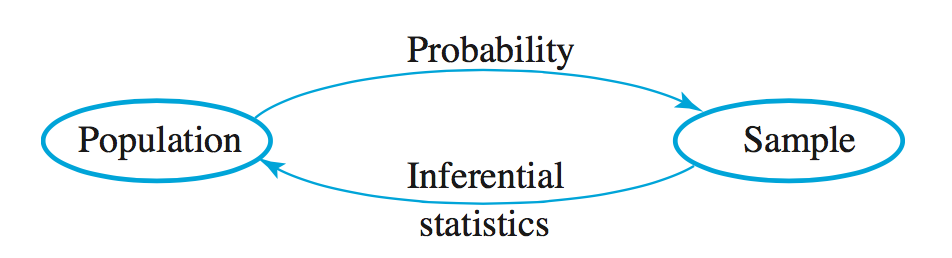
\includegraphics[width=0.8\linewidth,height=0.4\textheight]{images/probstats} \end{center}

If we know the characteristics of a population, the study of Probability will help us determine the likelihood that a sample will have certain characteristics.

Likewise, Statistics can potentially help us use the characteristics of a sample to say something about the population.

\newpage

\section{R Companion for Chapter 1}\label{r-companion-for-chapter-1}

\underline{Example 1:} Let's manually enter the heights data set (183, 170, 160, 175, 187) from chapter 1 and the following R commands will do the calculations we completed by hand.

\underline{Note:} Lines of code that begin with \textbf{\#} are comments and are not executed by the computer. Lines of code that begin with \textbf{\#} denote the output.

\begin{Shaded}
\begin{Highlighting}[]
\CommentTok{\# manually enter your data by using the "c" command}
\NormalTok{heights }\OtherTok{=} \FunctionTok{c}\NormalTok{(}\DecValTok{183}\NormalTok{,}\DecValTok{165}\NormalTok{,}\DecValTok{165}\NormalTok{,}\DecValTok{175}\NormalTok{,}\DecValTok{187}\NormalTok{)}

\CommentTok{\# calculate sample statistics on data set}
\FunctionTok{mean}\NormalTok{(heights)}
\end{Highlighting}
\end{Shaded}

\begin{verbatim}
## [1] 175
\end{verbatim}

\begin{Shaded}
\begin{Highlighting}[]
\FunctionTok{median}\NormalTok{(heights)}
\end{Highlighting}
\end{Shaded}

\begin{verbatim}
## [1] 175
\end{verbatim}

\begin{Shaded}
\begin{Highlighting}[]
\FunctionTok{var}\NormalTok{(heights)}
\end{Highlighting}
\end{Shaded}

\begin{verbatim}
## [1] 102
\end{verbatim}

\begin{Shaded}
\begin{Highlighting}[]
\FunctionTok{sd}\NormalTok{(heights)}
\end{Highlighting}
\end{Shaded}

\begin{verbatim}
## [1] 10.0995
\end{verbatim}

We can also create a histogram in R. Note that we can specify the breaks for the bins. In this case, the breaks are defined at 160, 170, 180, 190.

\begin{Shaded}
\begin{Highlighting}[]
\FunctionTok{hist}\NormalTok{(heights,}\AttributeTok{breaks=}\FunctionTok{c}\NormalTok{(}\DecValTok{160}\NormalTok{,}\DecValTok{170}\NormalTok{,}\DecValTok{180}\NormalTok{,}\DecValTok{190}\NormalTok{))}
\end{Highlighting}
\end{Shaded}

\begin{center}
\includegraphics[height=0.3\textheight]{_main_files/figure-latex/unnamed-chunk-20-1} \end{center}

\newpage

\underline{Example 2:} Let's create a randomized dataset of eye colors and analyze the data.

\underline{Note:} When we generate random data in this class, we will use the \textbf{set.seed} function, so that we all generate the same random data. If we don't use the \textbf{set.seed} command before generating random data, we will all get different random data.

Here, we generate 47 random eye colors and take a look at the first few observations.

\begin{Shaded}
\begin{Highlighting}[]
\FunctionTok{set.seed}\NormalTok{(}\DecValTok{2020}\NormalTok{)}
\NormalTok{eye.colors }\OtherTok{=} \FunctionTok{sample}\NormalTok{(}\FunctionTok{c}\NormalTok{(}\StringTok{"amber"}\NormalTok{, }\StringTok{"blue"}\NormalTok{, }\StringTok{"brown"}\NormalTok{, }\StringTok{"gray"}\NormalTok{, }\StringTok{"green"}\NormalTok{,}
                       \StringTok{"hazel"}\NormalTok{, }\StringTok{"red"}\NormalTok{), }\DecValTok{47}\NormalTok{, }\AttributeTok{replace =}\NormalTok{ T)}

\CommentTok{\# the "head" function will give the first few data values }
\CommentTok{\# or the "header" of the dataset}
\FunctionTok{head}\NormalTok{(eye.colors)}
\end{Highlighting}
\end{Shaded}

\begin{verbatim}
## [1] "gray"  "gray"  "red"   "hazel" "amber" "amber"
\end{verbatim}

We can create a frequency table of these values and create a barplot.

\begin{Shaded}
\begin{Highlighting}[]
\FunctionTok{table}\NormalTok{(eye.colors)}
\end{Highlighting}
\end{Shaded}

\begin{verbatim}
## eye.colors
## amber  blue brown  gray green hazel   red 
##     3    10     3    10     7     8     6
\end{verbatim}

\begin{Shaded}
\begin{Highlighting}[]
\FunctionTok{barplot}\NormalTok{(}\FunctionTok{table}\NormalTok{(eye.colors), }\AttributeTok{xlab =} \StringTok{"eye color"}\NormalTok{, }
        \AttributeTok{ylab =} \StringTok{"frequency"}\NormalTok{, }\AttributeTok{main =} \StringTok{"Bar plot of eye color occurance"}\NormalTok{)}
\end{Highlighting}
\end{Shaded}

\begin{center}
\includegraphics[height=0.4\textheight]{_main_files/figure-latex/unnamed-chunk-22-1} \end{center}

\newpage

We can also calculate proportion and percentage tables.

\begin{Shaded}
\begin{Highlighting}[]
\FunctionTok{table}\NormalTok{(eye.colors) }\CommentTok{\# shows how many of each value exist}
\end{Highlighting}
\end{Shaded}

\begin{verbatim}
## eye.colors
## amber  blue brown  gray green hazel   red 
##     3    10     3    10     7     8     6
\end{verbatim}

\begin{Shaded}
\begin{Highlighting}[]
\FunctionTok{length}\NormalTok{(eye.colors) }\CommentTok{\# tells how many data points there are}
\end{Highlighting}
\end{Shaded}

\begin{verbatim}
## [1] 47
\end{verbatim}

\begin{Shaded}
\begin{Highlighting}[]
\FunctionTok{table}\NormalTok{(eye.colors)}\SpecialCharTok{/}\FunctionTok{length}\NormalTok{(eye.colors) }\CommentTok{\# proportion}
\end{Highlighting}
\end{Shaded}

\begin{verbatim}
## eye.colors
##      amber       blue      brown       gray      green      hazel        red 
## 0.06382979 0.21276596 0.06382979 0.21276596 0.14893617 0.17021277 0.12765957
\end{verbatim}

\begin{Shaded}
\begin{Highlighting}[]
\FunctionTok{table}\NormalTok{(eye.colors)}\SpecialCharTok{/}\FunctionTok{length}\NormalTok{(eye.colors)}\SpecialCharTok{*}\DecValTok{100} \CommentTok{\# percent}
\end{Highlighting}
\end{Shaded}

\begin{verbatim}
## eye.colors
##     amber      blue     brown      gray     green     hazel       red 
##  6.382979 21.276596  6.382979 21.276596 14.893617 17.021277 12.765957
\end{verbatim}

\chapter{Probability}\label{probability}

In this chapter, we'll delve into Probability, the branch of mathematics that deals with the study of randomness and uncertainty, helping us understand and quantify the likelihood of different outcomes.

\section{Sample Space and Events}\label{sample-space-and-events}

\begin{definition}
An \textbf{\emph{experiment}} is any activity or process whose outcome is subject to uncertainty.
\end{definition}

\begin{definition}
The \textbf{\emph{sample space}} of an experiment, denoted by \(\Omega\) or \(\mathcal{S}\), is the set of all possible outcomes of that experiment.
\end{definition}

\begin{definition}
An \textbf{\emph{event}} is any collection (subset) of outcomes contained in the sample space \(\Omega\).
\end{definition}

\begin{example}
For the following examples, define the sample space and give an example of an event. Code for running the experiment in R is given.
\end{example}

\textbf{Experiment 1:} Roll a fair six-sided die.

\begin{Shaded}
\begin{Highlighting}[]
\CommentTok{\# roll one fair six{-}sided die in R}
\FunctionTok{sample}\NormalTok{(}\AttributeTok{x=}\DecValTok{1}\SpecialCharTok{:}\DecValTok{6}\NormalTok{,}\AttributeTok{size=}\DecValTok{1}\NormalTok{)}
\end{Highlighting}
\end{Shaded}

\begin{verbatim}
## [1] 5
\end{verbatim}

\textbf{Experiment 2:} Roll two fair six-sided dice.

\begin{Shaded}
\begin{Highlighting}[]
\CommentTok{\# roll two fair six{-}sided dice in R}
\FunctionTok{sample}\NormalTok{(}\AttributeTok{x=}\DecValTok{1}\SpecialCharTok{:}\DecValTok{6}\NormalTok{,}\AttributeTok{size=}\DecValTok{2}\NormalTok{)}
\end{Highlighting}
\end{Shaded}

\begin{verbatim}
## [1] 1 3
\end{verbatim}

\textbf{Experiment 3:} Randomly select a real number in the closed interval from 0 to 1.

\begin{Shaded}
\begin{Highlighting}[]
\CommentTok{\# generate one random number between 0 and 1}
\FunctionTok{runif}\NormalTok{(}\AttributeTok{n=}\DecValTok{1}\NormalTok{)}
\end{Highlighting}
\end{Shaded}

\begin{verbatim}
## [1] 0.6137196
\end{verbatim}

\newpage

\section{Set Theory}\label{set-theory}

\textbf{Note:} For the following examples, suppose a fair six-sided die is rolled, so \(\Omega=\{1,2,3,4,5,6\}\).

Define the following events: \(A = \text{roll an even} = \{2,4,6\}\), \(B=\text{roll a 3 or higher} =\{3,4,5,6\}\), \(C=\text{roll a prime number}=\{2,3,5\}\).

\begin{definition}
A \textbf{\emph{complement}} of an event A, denoted by \(A^c\) or A', is the set of all outcomes in \(\Omega\) that are not contained in A.
\end{definition}

\textbf{Illustration}

\begin{flushleft}
\includegraphics[height=0.1\textheight]{_main_files/figure-latex/unnamed-chunk-28-1} \end{flushleft}

\begin{definition}
The \textbf{\emph{union}} of two events A and B, denoted by \(A \cup B\) and read ``A or B'', is the event consisting of all outcomes that are either in A or B or in both.
\end{definition}

\textbf{Illustration}

\begin{flushleft}
\includegraphics[height=0.1\textheight]{_main_files/figure-latex/unnamed-chunk-29-1} \end{flushleft}

\begin{definition}
The \textbf{\emph{intersection}} of two events A and B, denoted by \(A \cap B\) and read ``A and B'', is the event consisting of all outcomes that are in both A and B.
\end{definition}

\textbf{Illustration}

\begin{flushleft}
\includegraphics[height=0.1\textheight]{_main_files/figure-latex/unnamed-chunk-31-1} \end{flushleft}

\begin{definition}
The \textbf{\emph{set difference}} of two events A and B, denoted by A\textbackslash B and read ``difference of A and B'', is the event consisting of all outcomes that are in A but not in B.
\end{definition}

\textbf{Illustration}

\begin{flushleft}
\includegraphics[height=0.1\textheight]{_main_files/figure-latex/unnamed-chunk-32-1} \end{flushleft}

\begin{definition}
The \textbf{\emph{null or empty set}} is the set of no events (or elements), denoted \(\emptyset\).
\end{definition}

\begin{definition}
When \(A \cap B = \emptyset\), A and B are said to be \textbf{\emph{mutually exclusive (or disjoint)}} events.
\end{definition}

\newpage

\begin{example}
Suppose a fair six-sided die is rolled, so \(\Omega=\{1,2,3,4,5,6\}\).

Define the following events: \(A = \text{roll an even} = \{2,4,6\}\), \(B=\text{roll a 3 or higher} =\{3,4,5,6\}\), \(C=\text{roll a prime number}=\{2,3,5\}\).

Determine the following sets and fill in the Venn diagrams representing these sets.
\end{example}

\begin{example}
Draw and determine \(A \cup B^c\).
\end{example}

\vfill

\begin{flushleft}
\includegraphics[height=0.15\textheight]{_main_files/figure-latex/unnamed-chunk-33-1} \end{flushleft}

\begin{example}
Draw and determine \(A \cap B \cap C^C\).
\end{example}

\vfill

\begin{flushleft}
\includegraphics[height=0.15\textheight]{_main_files/figure-latex/unnamed-chunk-34-1} \end{flushleft}

\begin{example}
Draw and determine \([A \cup B] \cap C\).
\end{example}

\vfill

\begin{flushleft}
\includegraphics[height=0.15\textheight]{_main_files/figure-latex/unnamed-chunk-35-1} \end{flushleft}

\begin{example}
Draw and determine \(A \cap B \cap C\).
\end{example}

\vfill

\begin{flushleft}
\includegraphics[height=0.15\textheight]{_main_files/figure-latex/unnamed-chunk-36-1} \end{flushleft}

\newpage

\section{Axioms and Rules of Probability}\label{axioms-and-rules-of-probability}

\begin{definition}
The probability of an event, \(A\), is denoted by \(P(A)\) and represents the likelihood or chance that the event \(A\) will occur. Note that \(0 \leq P(A) \leq 1\).
\end{definition}

\textbf{Axioms of Probability}

The axioms of probability were introduced by the mathematician Andrey Kolmogorov in 1933. These axioms form the foundation of probability theory, providing a rigorous, axiomatic framework for quantifying uncertainty. In mathematics, an axiomatic approach means that all rules and theorems are built from a set of fundamental principles, or axioms.

\textbf{Axiom 1:} For any event A, \(P(A) \ge 0\)

\textbf{Axiom 2:} \(P(\Omega) = 1\)

\textbf{Axiom 3:} If \(A_1, A_2, A_3, \dots\) is an infinite collection of disjoint events, then
\[P \big( \cup_{i=1}^{\infty} A_i \big) = P(A_1 \cup A_2 \cup A_3 \cup \dots) = \sum_{i=1}^{\infty} P(A_i)\]

\textbf{Probability Rules}

The following can be derived from the Axioms of Probability.

\vfill

\begin{enumerate}
\def\labelenumi{\arabic{enumi}.}
\tightlist
\item
  \(P(\emptyset) = 0\)
\end{enumerate}

\vfill

\begin{enumerate}
\def\labelenumi{\arabic{enumi}.}
\setcounter{enumi}{1}
\tightlist
\item
  For any event A, \(P(A) + P(A^c)\) = 1
\end{enumerate}

\vfill

\begin{enumerate}
\def\labelenumi{\arabic{enumi}.}
\setcounter{enumi}{2}
\tightlist
\item
  \(P(A^c) = 1 - P(A)\)
\end{enumerate}

\vfill

\begin{enumerate}
\def\labelenumi{\arabic{enumi}.}
\setcounter{enumi}{3}
\tightlist
\item
  For any event A, \(0 \le P(A) \le 1\)
\end{enumerate}

\vfill

\begin{enumerate}
\def\labelenumi{\arabic{enumi}.}
\setcounter{enumi}{4}
\tightlist
\item
  For any two events A and B,
  \(P(A \cup B) = P(A) + P(B) - P(A \cap B)\)
\end{enumerate}

\vfill

\begin{enumerate}
\def\labelenumi{\arabic{enumi}.}
\setcounter{enumi}{5}
\tightlist
\item
  For any three events A, B, and C,
\end{enumerate}

\(P(A \cup B \cup C) = P(A) + P(B) + P(C) - P(A \cap B) - P(A \cap C) - P(B \cap C) + P(A \cap B \cap C)\).

\vfill

\begin{enumerate}
\def\labelenumi{\arabic{enumi}.}
\setcounter{enumi}{6}
\tightlist
\item
  \(\left[A \cup B\right]^C = A^C \cap B^C\)
\end{enumerate}

\vfill

\begin{enumerate}
\def\labelenumi{\arabic{enumi}.}
\setcounter{enumi}{7}
\tightlist
\item
  \(\left[A \cap B\right]^C = A^C \cup B^C\)
\end{enumerate}

\newpage

\begin{example}
Suppose our class has the following breakdown:

70\% Math students\\
20\% seniors\\
30\% Born in Denver\\
10\% Math students and seniors\\
15\% Math students and born in Denver\\
10\% Seniors and Born in Denver\\
5\% Math students, seniors, and born in Denver\\

Define events as follows: A = Math student, B = senior, C = Born in Denver.

Suppose a random student from the class is selected. Calculate the following probabilities.
\end{example}

\begin{enumerate}
\def\labelenumi{(\alph{enumi})}
\item
  \(P(A \cup B)\)
  \vfill
\item
  \(P(C \backslash B)\)
  \vfill
\item
  \(P([A \cap C]^c)\)
  \vfill
\item
  \(P(A \cup B \cup C)\)
  \vfill
\end{enumerate}

\newpage

\section{Counting Techniques}\label{counting-techniques}

\textbf{Equally Likely Outcomes}

If \(\Omega = \lbrace x_1, x_2, ... x_N \rbrace\) and all outcomes are equally likely, then \(P(A) = |A| / N\), where \(|A|\) is the number of outcomes contained in the event A.

\begin{example}
You roll a fair six-sided die. Calculate \(P(even)\).
\end{example}

\vfill

\begin{theorem}
(Product Rule for Ordered Pairs) If the first element of an ordered pair can be selected in \(n_1\) ways and for each of the these \(n_1\) ways the second element of the pair can be selected in \(n_2\) ways, then the number of pairs is \(n_1 \cdot n_2\).
\end{theorem}

\begin{example}
You flip two fair coins. Calculate the probability that all are heads or all are tails.
\end{example}

\vfill

\begin{theorem}
(Generalized Product Rule) Suppose a set consists of k elements (k-tuples) and that there are \(n_1\) possible choices for the first element, \(n_2\) possible choices for the second element, \ldots{} , and \(n_k\) possible choices for the \(k^{th}\) element, then there are \(n_1 \cdot n_2 \cdot \cdots n_k\) possible k-tuples.
\end{theorem}

\begin{example}
\leavevmode

Quartiles is a word game where one of the goals is to find all five words that contain four tiles each. Suppose we have found 3 of the quartiles. How many total attempts are there to find the fourth quartile?

\end{example}

\begin{center}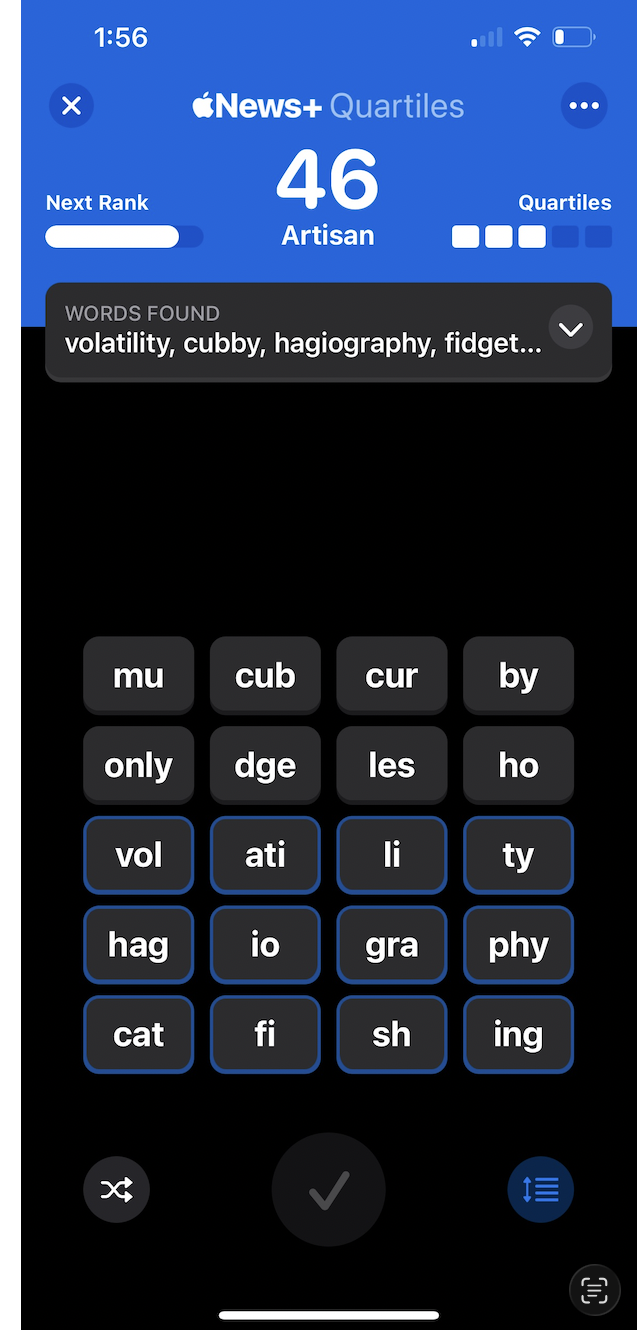
\includegraphics[width=0.8\linewidth,height=0.4\textheight]{images/QuartileExample} \end{center}
\vfill

\newpage

The factorial function, \(n!\), is important in counting methods and probability. It is the product of all positive integers less than or equal to \(n\), that is, \(n! =n \cdot (n-1) \cdot (n-2) \cdot \ldots \cdot 2 \cdot 1 \text{ for } n \in \mathbb{Z}^+\).

\textbf{Note:} \(0! = 1\)

\begin{definition}
An ordered subset is called a \textbf{\emph{permutation}}. The number of permutations of size \(k\) that can be formed from the \(n\) elements in a set will be denoted by \(P_{n,k}\).

\(\boxed{P_{n,k} = \frac{n!}{(n-k)!}}\)
\end{definition}

\begin{definition}
An unordered subset is called a \textbf{\emph{combination}}. The number of combinations of size \(k\) that can be formed from the \(n\) elements in a set will be denoted by \(\binom{n}{k}\) or \(C_{n,k}\).

\(\boxed{\binom{n}{k} = C_{n,k} = \frac{n!}{k! \cdot (n-k)!}}\)
\end{definition}

\begin{example}
Suppose there are five competitors in an Olympic competition. A gold, a silver, and a bronze medal are awarded for the top three competitors. Are combinations or permutations more appropriate for this situation? How many possible ways can these three awards be given out?
\end{example}

\vfill

\begin{example}
Suppose there are five competitors in an Olympic competition and only three can advance to the final competition. Are combinations or permutations more appropriate for this situation? How many possible ways can you choose three people from a group of five?
\end{example}

\vfill

\newpage

\section{Conditional Probability}\label{conditional-probability}

Conditional probability is the likelihood of an event occurring given that another event has already occurred. It refines our understanding of probability by taking into account additional information that might affect the outcome. Understanding conditional probabilities is crucial in many areas of statistics and decision-making, as it allows us to update our predictions and assessments based on new evidence.

\begin{definition}
For any two events A and B with \(P(B)>0\), the \underline{conditional probability of A given B} is defined by:
\[P(A|B) = \frac{P(A \cap B)}{P(B)}\]
\end{definition}

\vfill

\begin{example}
The following is a contingency table from a survey on congressional approval.
\end{example}

\begin{longtable}[]{@{}
  >{\centering\arraybackslash}p{(\linewidth - 6\tabcolsep) * \real{0.2987}}
  >{\centering\arraybackslash}p{(\linewidth - 6\tabcolsep) * \real{0.2857}}
  >{\centering\arraybackslash}p{(\linewidth - 6\tabcolsep) * \real{0.3247}}
  >{\centering\arraybackslash}p{(\linewidth - 6\tabcolsep) * \real{0.0909}}@{}}
\toprule\noalign{}
\begin{minipage}[b]{\linewidth}\centering
Political Affiliation
\end{minipage} & \begin{minipage}[b]{\linewidth}\centering
Approves of Congress
\end{minipage} & \begin{minipage}[b]{\linewidth}\centering
Disapproves of Congress
\end{minipage} & \begin{minipage}[b]{\linewidth}\centering
Total
\end{minipage} \\
\midrule\noalign{}
\endhead
\bottomrule\noalign{}
\endlastfoot
Republican & 100 & 20 & 120 \\
Democrat & 20 & 80 & 100 \\
Independent & 40 & 40 & 80 \\
Total & 160 & 140 & 300 \\
\end{longtable}

\begin{enumerate}
\def\labelenumi{(\alph{enumi})}
\tightlist
\item
  What is the probability that a randomly selected individual from the survey approves of Congress?
\end{enumerate}

\vfill

\begin{enumerate}
\def\labelenumi{(\alph{enumi})}
\setcounter{enumi}{1}
\tightlist
\item
  What is the probability that a randomly selected individual approves of Congress given that they are Democrat?
\end{enumerate}

\vfill

\begin{enumerate}
\def\labelenumi{(\alph{enumi})}
\setcounter{enumi}{2}
\tightlist
\item
  Given that the randomly selected person approves of the Congress, what is the probability that they are Republican?
\end{enumerate}

\vfill

\newpage

\begin{theorem}
Multiplication Rule: \(P(A \cap B) = P(A|B) \cdot P(B)\)
\end{theorem}

\begin{example}
Suppose that people with a genetic variation have a 50\% chance of getting a rare disease. The probability of having the genetic variation is 1\%. What is the probability that a randomly chosen person has the genetic variation and also has the disease?
\end{example}

\vfill

\begin{theorem}
Law of Total Probability: Let \(A_1, A_2, \ldots, A_k\) be mutually exclusive and exhaustive events (i.e., the events form a partition). Then for any event B,
\[P(B) = P(B|A_1) \cdot P(A_1) + P(B|A_2) \cdot P(A_2) + \ldots + P(B|A_k) \cdot P(A_k) \]
\end{theorem}

\textbf{Illustration of a Partition}

\begin{center}
\includegraphics[height=0.4\textheight]{_main_files/figure-latex/unnamed-chunk-39-1} \end{center}

\vfill

\newpage

\begin{example}
Box \#1 has ten computer chips (five working and five broken). Box \#2 has five (one working and four broken). Suppose we randomly select one of the two boxes and then randomly select a chip. What is the probability that the chip is broken?
\end{example}

\vfill

\begin{theorem}
Bayes' Theorem: Suppose that \(A_1 \cap A_2 = \emptyset\) and \(A_1 \cup A_2 = \Omega\), then if \(P(B)>0\),

\[ P(A_1|B) = \frac{P(B|A_1)P(A_1)}{P(B|A_1)P(A_1)+P(B|A_2)P(A_2)} \]

\smallskip

Let \(A_1, A_2, \ldots, A_k\) be a collection of mutually exclusive and exhaustive events, then if \(P(B)>0\),

\[P(A_j|B) = \frac{P(A_j \cap B)}{P(B)} = \frac{P(B|A_j) \cdot P(A_j)}{\sum_{i=1}^k P(B|A_i) \cdot P(A_i)}
\]
\end{theorem}

\smallskip

\begin{example}
Suppose a test to detect a rare disease is positive 95\% of the time for a person with a disease and is positive 1\% of the time for a person without the disease. Further, assume that 0.5\% of the population has the disease. Given that a person tests positive for a disease, what is the probability that they actually has the disease?
\end{example}

\vfill

\newpage

\section{Independence}\label{independence}

Recall:

\begin{definition}
When \(A \cap B = \emptyset\), A and B are said to be \textbf{\emph{mutually exclusive (or disjoint)}} events.
\end{definition}

\begin{definition}
Two events A and B are \textbf{\emph{independent}} if \(P(A|B) = P(A)\) and \textbf{\emph{dependent}} otherwise.

Also, A and B are independent if and only if \(P(A \cap B) = P(A) \cdot P(B)\).
\end{definition}

\begin{example}
Recall from the previous example that a test to detect a rare disease is positive 95\% of the time for a person with a disease and is positive 1\% of the time for a person without the disease. Further, assume that 0.5\% of the population has the disease. Let \(D\) be the event that one has the disease and let \(P\) be the event that one has a positive test.
\end{example}

\begin{enumerate}
\def\labelenumi{(\alph{enumi})}
\item
  Are D and P mutually exclusive?
  \vfill
\item
  Are D and P independent?
  \vfill
\end{enumerate}

\section{Objective vs.~Subjective Probability}\label{objective-vs.-subjective-probability}

There are two different interpretations of Probability. Both follow the Axioms of Probability.

\begin{definition}
\textbf{\emph{Objective Probability}} refers to the probability of an event as determined by the long-term frequency of its occurrence, based on repeated trials or observations. It is rooted in empirical data and reflects the likelihood of an event as the proportion of times it occurs in a large number of trials.
\end{definition}

\begin{example}
I flip a coin 100 times and it lands on head 53 times. I estimate the probability of flipping a heads to be \(P_{100}(head) = \frac{53}{100} = 0.53\). As we flip the coin more and more, we would expect that \(P_n(head) \to 0.5\) as \(n \to \infty\) if the coin is actually a fair coin.
\end{example}

\begin{definition}
\textbf{\emph{Subjective Probability}} refers to the probability of an event as determined by an individual's personal judgment or belief, rather than objective data. It reflects the degree of confidence one has in the occurrence of an event. A well-known approach to subjective probability is Bayesian probability, which updates these beliefs based on new evidence.
\end{definition}

\begin{example}
I am given a coin which I have no reason to believe it is unfair (i.e, \(P(head) = 0.5\)). I flip the coin 100 times and 3 land on heads. Since this is very unlikely to happen if the coin is fair, I update my estimate to be \(P(head)=0.1\) (i.e., somewhere in between \(3/100=0.03\) and \(1/2 = 0.5\)).
\end{example}

\newpage

\section{R Companion for Chapter 2}\label{r-companion-for-chapter-2}

\begin{example}
Let's simulate a fair six-sided die roll. Recall that we need to use the \textbf{set.seed} function so that we all generate the same random data. For consistency, I always set the seed to 2020, i.e., set.seed(2020). The sample function will generate 100 random die rolls with each possible outcome (1,2,3,4,5,6) being equally likely.
\end{example}

\begin{Shaded}
\begin{Highlighting}[]
\FunctionTok{set.seed}\NormalTok{(}\DecValTok{2020}\NormalTok{)}
\NormalTok{data }\OtherTok{=} \FunctionTok{sample}\NormalTok{(}\AttributeTok{x =} \DecValTok{1}\SpecialCharTok{:}\DecValTok{6}\NormalTok{,}\AttributeTok{size =} \DecValTok{100}\NormalTok{,}\AttributeTok{replace =}\NormalTok{ T); data}
\end{Highlighting}
\end{Shaded}

\begin{verbatim}
##   [1] 4 4 6 1 1 4 2 6 1 5 2 2 6 5 2 3 2 5 4 2 6 6 4 6 4 2 4 5 4 4 3 6 2 2 6 3 5 4 5 5 2 5 1 6 3 5 1 5 3 1 5
##  [52] 3 2 6 2 1 3 2 1 6 5 5 2 5 6 4 3 6 4 4 2 2 1 6 1 4 6 2 2 2 1 4 1 1 4 2 2 5 5 4 4 4 6 5 4 1 6 5 1 4
\end{verbatim}

Let's make a histogram of the simulated data. Recall that each outcome (1,2,3,4,5,6) is equally likely in theory but in our simulation, some numbers may come up more than others. To make the histogram look better, I define the boundary breaks to be 0:6 (i.e., 0,1,2,3,4,5,6).

\begin{Shaded}
\begin{Highlighting}[]
\FunctionTok{hist}\NormalTok{(data,}\AttributeTok{breaks=}\DecValTok{0}\SpecialCharTok{:}\DecValTok{6}\NormalTok{)}
\end{Highlighting}
\end{Shaded}

\begin{center}
\includegraphics[height=0.4\textheight]{_main_files/figure-latex/unnamed-chunk-41-1} \end{center}

With only 100 random die rolls, the distribution isn't as flat, uniform, and symmetric as we would expect. The number 3 came up less than we would anticipate. This is OK.

\newpage

We can also generate a frequency table and use this to create a barplot. This looks a little nicer than the standard histogram and doesn't require use to use the \textbf{breaks} argument.

\begin{Shaded}
\begin{Highlighting}[]
\FunctionTok{table}\NormalTok{(data)}
\end{Highlighting}
\end{Shaded}

\begin{verbatim}
## data
##  1  2  3  4  5  6 
## 15 21  8 21 18 17
\end{verbatim}

\begin{Shaded}
\begin{Highlighting}[]
\FunctionTok{barplot}\NormalTok{(}\FunctionTok{table}\NormalTok{(data))}
\end{Highlighting}
\end{Shaded}

\begin{center}
\includegraphics[height=0.4\textheight]{_main_files/figure-latex/unnamed-chunk-42-1} \end{center}

If we want a better representation of the true distribution of the fair six-sided die rolls, we could simulate 10000 die rolls instead of 100.

\begin{Shaded}
\begin{Highlighting}[]
\FunctionTok{set.seed}\NormalTok{(}\DecValTok{2020}\NormalTok{)}
\NormalTok{data }\OtherTok{=} \FunctionTok{sample}\NormalTok{(}\AttributeTok{x =} \DecValTok{1}\SpecialCharTok{:}\DecValTok{6}\NormalTok{,}\AttributeTok{size =} \DecValTok{10000}\NormalTok{,}\AttributeTok{replace =}\NormalTok{ T)}
\FunctionTok{table}\NormalTok{(data)}
\end{Highlighting}
\end{Shaded}

\begin{verbatim}
## data
##    1    2    3    4    5    6 
## 1630 1657 1733 1655 1629 1696
\end{verbatim}

\newpage

\begin{Shaded}
\begin{Highlighting}[]
\FunctionTok{barplot}\NormalTok{(}\FunctionTok{table}\NormalTok{(data))}
\end{Highlighting}
\end{Shaded}

\begin{center}
\includegraphics[width=0.75\linewidth,height=0.4\textheight]{_main_files/figure-latex/unnamed-chunk-44-1} \end{center}

Simulation can be helpful for us to verify hand calculations and to estimate quantities that are hard to calculate by hand. Our simulation results won't exactly match our hand calculations, but if the sample size is large enough, they should be close.\textbackslash{}

For instance, we know that P(Roll=1) = 1/6 for the population of all fair six-sided die rolls. If you refer to the table at the bottom of the previous page, you see that 1 came up 1630 times out of 10000 die rolls. In the simulation, P(1) = 1630/10000 = 0.1630 which is pretty close the the theoretical value of P(1) = 1/6 = 0.1667.\textbackslash{}

Here is an example of how to calculate the probability of a die roll less than 3 in our simulation.

\begin{Shaded}
\begin{Highlighting}[]
\CommentTok{\# Calculate P(Roll \textless{} 3)}
\CommentTok{\# From theory, we know that P(Roll \textless{} 3) = P(1) + P(2) = 1/6 + 1/6 = 1/3}

\CommentTok{\# count up the number of rolls less than 3}
\NormalTok{num.under3 }\OtherTok{=} \FunctionTok{sum}\NormalTok{( data }\SpecialCharTok{\textless{}} \DecValTok{3}\NormalTok{ ) }

\CommentTok{\# divide the number of rolls less than 3 by the number of rolls}
\NormalTok{prob.under3 }\OtherTok{=}\NormalTok{ num.under3 }\SpecialCharTok{/} \DecValTok{10000}
\NormalTok{prob.under3}
\end{Highlighting}
\end{Shaded}

\begin{verbatim}
## [1] 0.3287
\end{verbatim}

\begin{Shaded}
\begin{Highlighting}[]
\CommentTok{\# alternatively:}
\NormalTok{prob.under3 }\OtherTok{=} \FunctionTok{mean}\NormalTok{(data }\SpecialCharTok{\textless{}} \DecValTok{3}\NormalTok{)}
\NormalTok{prob.under3}
\end{Highlighting}
\end{Shaded}

\begin{verbatim}
## [1] 0.3287
\end{verbatim}

From theory, we expect P(Roll \(<\) 3) = 1/3 = 0.3333. In our simulation, we found P(Roll \(<\) 3) = 0.3287.

\newpage

\begin{example}
Let's simulate rolling two fair six-sided dice 10,000 times and calculate some probabilities. \textbf{d1} will represent the first die roll and \textbf{d2} will represent the second die roll.
\end{example}

\begin{Shaded}
\begin{Highlighting}[]
\FunctionTok{set.seed}\NormalTok{(}\DecValTok{2020}\NormalTok{)}
\NormalTok{d1 }\OtherTok{=} \FunctionTok{sample}\NormalTok{(}\AttributeTok{x =} \DecValTok{1}\SpecialCharTok{:}\DecValTok{6}\NormalTok{,}\AttributeTok{size =} \DecValTok{10000}\NormalTok{,}\AttributeTok{replace =}\NormalTok{ T)}
\NormalTok{d2 }\OtherTok{=} \FunctionTok{sample}\NormalTok{(}\AttributeTok{x =} \DecValTok{1}\SpecialCharTok{:}\DecValTok{6}\NormalTok{,}\AttributeTok{size =} \DecValTok{10000}\NormalTok{,}\AttributeTok{replace =}\NormalTok{ T)}
\end{Highlighting}
\end{Shaded}

From our simulated data, let's calculate P(D1 = 1 and D2 = 2), that is, the probability that first die roll is 1 and the second die roll is 2. From theory, this probability should be 1/36 = 0.0278. (We use the \textbf{\&} for \textbf{AND} in R.)

\begin{Shaded}
\begin{Highlighting}[]
\NormalTok{num.events }\OtherTok{=} \FunctionTok{sum}\NormalTok{(d1 }\SpecialCharTok{==} \DecValTok{1} \SpecialCharTok{\&}\NormalTok{ d2 }\SpecialCharTok{==} \DecValTok{2}\NormalTok{)}
\NormalTok{prob }\OtherTok{=}\NormalTok{ num.events }\SpecialCharTok{/} \DecValTok{10000}\NormalTok{; prob}
\end{Highlighting}
\end{Shaded}

\begin{verbatim}
## [1] 0.0256
\end{verbatim}

Next, let's calculate P(D1 \(<\) 2 or D2 \(>\) 2), that is, the probability that the first die roll is less than 2 or the second die roll is greater than 2. From theory, this probability should be 0.7222. We use the \textbf{$\vert$} for the \textbf{OR} in R.)

\begin{Shaded}
\begin{Highlighting}[]
\NormalTok{num.events }\OtherTok{=} \FunctionTok{sum}\NormalTok{(d1 }\SpecialCharTok{\textless{}} \DecValTok{2} \SpecialCharTok{|}\NormalTok{ d2 }\SpecialCharTok{\textgreater{}} \DecValTok{2}\NormalTok{)}
\NormalTok{prob }\OtherTok{=}\NormalTok{ num.events }\SpecialCharTok{/} \DecValTok{10000}\NormalTok{; prob}
\end{Highlighting}
\end{Shaded}

\begin{verbatim}
## [1] 0.7183
\end{verbatim}

Finally, let's look at the frequency table and distribution of the sum of the two die rolls.

\begin{Shaded}
\begin{Highlighting}[]
\FunctionTok{table}\NormalTok{(d1}\SpecialCharTok{+}\NormalTok{d2)}
\end{Highlighting}
\end{Shaded}

\begin{verbatim}
## 
##    2    3    4    5    6    7    8    9   10   11   12 
##  271  540  824 1154 1373 1703 1360 1149  814  525  287
\end{verbatim}

\begin{Shaded}
\begin{Highlighting}[]
\FunctionTok{barplot}\NormalTok{(}\FunctionTok{table}\NormalTok{(d1}\SpecialCharTok{+}\NormalTok{d2),}\AttributeTok{xlab=}\StringTok{"Sum of Dice"}\NormalTok{,}\AttributeTok{ylab=}\StringTok{"Counts"}\NormalTok{)}
\end{Highlighting}
\end{Shaded}

\begin{center}
\includegraphics[width=0.7\linewidth,height=0.4\textheight]{_main_files/figure-latex/unnamed-chunk-49-1} \end{center}

\chapter{Discrete Random Variables}\label{discrete-random-variables}

In this chapter, we'll explore random variables and their associated probability distributions, with a focus on discrete random variables. These concepts are the backbone of probability theory, enabling us to model and analyze uncertainty. We'll also briefly cover the differences between discrete and continuous random variables---discrete variables take on specific, countable values, while continuous variables can assume any value within a range.

\section{Random Variables}\label{random-variables}

\begin{definition}
For a given sample space \(\Omega\) of an experiment, a \textbf{\emph{random variable (RV)}} is a rule that assigns a number to each outcome in \(\Omega\). Mathematically, a random variable is a function with the sample space as its domain and the set of real numbers as its range.
\end{definition}

\begin{definition}
A \textbf{\emph{discrete random variable}} is a random variable whose possible values either constitute a finite set or a countably infinite set.
\end{definition}

\begin{definition}
A \textbf{\emph{continuous}} random variable is a random variable whose possible values are uncountably infinite or defined over an interval. Note: \(P(X=c)=0\) for a continuous random variable \(X\) and a constant \(c\).
\end{definition}

\begin{example}
For the following cases, determine whether the random variable is discrete or continuous and state the sample space, \(\Omega\).
\end{example}

\begin{enumerate}
\def\labelenumi{(\alph{enumi})}
\item
  Roll a fair six-sided die. Let \(X\) be the number on the top of the die.
  \vfill
\item
  Pick a random person and let \(Y\) be the number of keys in their pocket.
  \vfill
\item
  Suppose a student is given 50 minutes to complete an exam. Let \(Z\) be the amount of time it takes the student to complete the exam.
  \vfill
\end{enumerate}

\newpage

\section{Probability Distributions for Discrete Random Variables}\label{probability-distributions-for-discrete-random-variables}

\begin{definition}
The \textbf{\emph{probability mass function (pmf)}} or \textbf{\emph{probability distribution}} of a discrete random variable \(X\) is defined for every number \(x\) by \(p(x) = P(X=x)\).

\textbf{Note:} \(\sum_{x \in X} p(x) = 1\)
\end{definition}

\begin{definition}

The \textbf{\emph{cumulative distribution function (CDF)}} \(F(x)\) of a discrete random variable \(X\) with pmf \(p(x)\) is defined for every number x by:
\(F(x) = P(X \le x) = \sum_{y:y \le x} p(y)\)

\begin{itemize}
\item
  \(F(x)\) gives you the probability that a random variable will be at most equal to \(x\).
\item
  \(F(x)\) must be right-continuous and non-decreasing.
\item
  \(F(x)\) must satisfy two limit laws:

  \begin{itemize}
  \tightlist
  \item
    \begin{enumerate}
    \def\labelenumi{(\roman{enumi})}
    \tightlist
    \item
      \(\lim_{x \to -\infty} F(x) = 0\)\\
    \end{enumerate}
  \item
    \begin{enumerate}
    \def\labelenumi{(\roman{enumi})}
    \setcounter{enumi}{1}
    \tightlist
    \item
      \(\lim_{x \to \infty} F(x) = 1\)\\
    \end{enumerate}
  \end{itemize}
\end{itemize}

\end{definition}

\begin{theorem}
For any two numbers a and b with \(a \le b\), \(P(a \le X \le b ) = F(b) - F(a^-)\).
\end{theorem}

\begin{example}
Roll a fair six-sided die. Let \(X\) be the number of the top of the die. Find the pmf and cdf of \(X\) and sketch them.
\end{example}

\vfill

\begin{center}
\includegraphics[width=0.9\linewidth,height=0.4\textheight]{_main_files/figure-latex/unnamed-chunk-52-1} \end{center}

\vfill
\vfill
\vfill
\vfill
\vfill

\newpage

\vfill

\begin{example}
Flip two fair coins. Let \(Y\) be the number of coins that land on heads. Find the pmf and cdf of \(Y\) and sketch both.
\end{example}

\vfill

\begin{center}
\includegraphics[width=0.7\linewidth,height=0.4\textheight]{_main_files/figure-latex/unnamed-chunk-53-1} \end{center}

\vfill
\vfill
\vfill
\vfill
\vfill

\section{Expected Values (Means)}\label{expected-values-means}

\begin{definition}
Let X be a discrete random variable with set of possible outcomes \(D\) and pmf \(p(x)\). The \textbf{\emph{expected value}} or \textbf{\emph{mean value}} of \(X\), denoted \(E[X]\) or \(\mu\), is: \[E[X] = \sum_{x \in D} x \cdot p(x)\]
\end{definition}

\begin{theorem}
\(E[h(X)] = \sum p(x) \cdot h(x)\)
\end{theorem}

\begin{theorem}
\(E[aX+b] = a \cdot E[X] + b\)
\end{theorem}

\begin{definition}
Let X have a pmf \(p(x)\) and expected value \(\mu\). Then the \textbf{\emph{variance}} of X, denoted by \(Var(X)\) or \(\sigma^2\), is:
\[Var(X) = \sigma^2 = \sum_{x \in D} (x-\mu)^2 \cdot p(x) = E[(X-\mu)^2]\]
\end{definition}

\begin{definition}
The \textbf{\emph{standard deviation}}, denoted SD or \(\sigma\) is:
\[SD(X) = \sigma  = \sqrt{Var(X)}\]
\end{definition}

\begin{theorem}
\(Var(X) = E[X^2] - (E[X])^2\)
\end{theorem}

\begin{theorem}
\(Var(aX+b) = a^2 \cdot \sigma^2\)
\end{theorem}

\newpage

\begin{example}
Roll a fair six-sided die. Let \(X\) be the number of the top of the die.
Find \(E[X]\) and \(Var(X)\).
\end{example}

\begin{table}[!h]
\centering
\begin{tabular}{c|c|c|c|c|c|c|c}
\hline
$x$ & 1 & 2 & 3 & 4 & 5 & 6 & $\Sigma$\\
\hline
$p(x)$ &  &  &  &  &  &  & \\
\hline
$x*p(x)$ &  &  &  &  &  &  & \\
\hline
$x^2*p(x)$ &  &  &  &  &  &  & \\
\hline
\end{tabular}
\end{table}

\begin{example}
Flip two fair coins. Let \(Y\) be the number of coins that land on heads. Find \(E[Y]\) and \(Var(Y)\).
\end{example}

\begin{table}[!h]
\centering
\begin{tabular}{c|c|c|c|c}
\hline
$y$ & 0 & 1 & 2 & $\Sigma$\\
\hline
$p(y)$ &  &  &  & \\
\hline
$y*p(y)$ &  &  &  & \\
\hline
$y^2*p(y)$ &  &  &  & \\
\hline
\end{tabular}
\end{table}

\begin{example}
Suppose \(Z = 3 \cdot Y + 2\), where \(Y\) is defined above. Find \(E[Z]\) and \(Var(Z)\).
\end{example}

\newpage

\section{Bernoulli and Binomial Random Variables}\label{bernoulli-and-binomial-random-variables}

\begin{definition}
Suppose \(p(x)\) depends on a quantity that can be assigned any one of a number of possible values, with each different value determining a different probability distribution. Such a quantity is called a \textbf{\emph{parameter}} of the distribution.
\end{definition}

\begin{definition}
The collection of all probability distributions for different values of the parameter is called a \textbf{\emph{family}} of probability distributions.
\end{definition}

\begin{definition}
A \textbf{\emph{Bernoulli(\(p\))}} random variable \(X\) is a discrete random variable with two possible outcomes (typically, these outcomes are 0 and 1).

The PMF of a Bernoulli(\(p\)) is:

\begin{flushleft}
$p(x) = \begin{cases}
1-p & x=0\\
p & x=1
\end{cases}$
\end{flushleft}

If \(X \sim \text{Bernoulli(}p)\)) random variable, then \(E[X] = p\) and \(Var(X) = p(1-p)\)
\end{definition}

\begin{example}
Show that if \(X\) is a Bernoulli(\(p\)) random variable, then \(E[X] = p\) and \(Var(X) = p(1-p)\).
\end{example}

\vfill

\begin{definition}
\leavevmode

\(X\) is a \textbf{\emph{Binomial(\(n\),\(p\))}} random variable if \(X\) is a discrete random variable that satisfies the following conditions:

\begin{itemize}
\item The experiment consists of $n$ Bernoulli trials, where $n$ is fixed.
\item The trials are independent.
\item The probability of success, $p$, is constant from trial to trial.
\item $X$ is the number of successes
\end{itemize}

The PMF of a Binomial(\(n,p\)) is:

\(p(x) = \binom{n}{x} p^x (1-p)^{n-x}, x = 0, 1, 2, \ldots, n\)

If \(X \sim \text{Binomial(}n,p)\) random variable, then \(E[X] = np\) and \(Var(X) = np(1-p)\).

\end{definition}

\newpage

\begin{example}
Basketball player Lebron James has a career free throw percentage of 73.1\% (i.e., there's a 73.1\% chance he will make a basket from the free throw line). Suppose Lebron has six free throw attempts in a game and assume all free throw shots are independent. Answer the following questions.
\end{example}

\begin{enumerate}
\def\labelenumi{(\alph{enumi})}
\tightlist
\item
  Let \(X\) be the number of free throws that Lebron makes. Find and sketch the pmf of \(X\).
\end{enumerate}

\begin{table}[!h]
\centering
\begin{tabular}{c|c|c|c|c|c|c|c}
\hline
$x$ & 0 & 1 & 2 & 3 & 4 & 5 & 6\\
\hline
$p(x)$ &  &  &  &  &  &  & \\
\hline
\end{tabular}
\end{table}

\begin{flushright}
\includegraphics[width=2in,height=0.4\textheight]{_main_files/figure-latex/unnamed-chunk-57-1} \end{flushright}

\begin{enumerate}
\def\labelenumi{(\alph{enumi})}
\tightlist
\item
  On average, how many free throws is Lebron expected to make? What is the variance?
\end{enumerate}

\vfill

\begin{enumerate}
\def\labelenumi{(\alph{enumi})}
\setcounter{enumi}{2}
\tightlist
\item
  What is the probability that Lebron makes at least five shots?
\end{enumerate}

\vfill

\newpage

\section{Geometric, Discrete Uniform, and Poisson Random Variables}\label{geometric-discrete-uniform-and-poisson-random-variables}

\begin{definition}
\(X\) is a \textbf{\emph{Geometric(\(p\))}} random variable is \(X\) is a discrete random variable with the following properties.

\begin{itemize}
\item The experiment consists of independent trials.
\item Each trial can result in a success or a failure.
\item The probability of success is $p$ and is constant across all trials.
\item The experiment continues until a successful trial is observed.
\item $X$ is the number of total trials
\end{itemize}

The PMF of a Geometric(\(p\)) is:

\(p(x) = p(1-p)^{x-1}, x = 1, 2, 3, \ldots\)

If \(X \sim \text{Geometric(}p)\) random variable, then \(E[X] = \frac{1}{p}\) and \(Var(X) = \frac{1-p}{p^2}\).
\end{definition}

\begin{example}
Basketball player Lebron James has a career free throw percentage of 73.1\%. Suppose he takes shots until makes one. Calculate the probability that 3 or more shots will be required to make his first shot.
\end{example}

\newpage

\begin{definition}
\(X\) is a \textbf{\emph{Discrete Uniform(a,b)}} random variable is \(X\) is a discrete random variable such that the outcomes \(a, a+1, \ldots, b\) are equally likely. Let \(n = b-a+1\).

The PMF of a Uniform(\(a,b\)) is:

\(p(x) = \frac{1}{n}, x = a, a+1, \ldots, b\)

If \(X \sim \text{Uniform(}a,b)\) random variable, then \(E[X] = \frac{a+b}{2}\) and \(Var(X) = \frac{(b-a+1)^2-1}{12}\).
\end{definition}

\begin{example}
Using the formulas above, calculate the expected value and variance of a fair six-sided die roll.
\end{example}

\vfill

\begin{definition}
A \textbf{\emph{Poisson random variable}} is a discrete random variable with parameter \(\lambda\) and the following pmf: \[p(x)=\frac{e^{-\lambda} \lambda^x}{x!}, x = 0, 1, 2, \ldots \]

If \(X \sim \text{Poisson(}\lambda)\) random variable, then \(E[X] = \lambda\) and \(Var(X) = \lambda\).
\end{definition}

\textbf{Note:} Poisson random variables are often used to model the number of events that occur in a finite period of time.

\begin{example}
Jihan is going fishing and on average, she catches 2 fish per day. Assume that the time between successive fish caught is independent. What is the probability that Jihan catches less than 3 fish in a given day?
\end{example}

\vfill

\newpage

\section{R Companion for Chapter 3}\label{r-companion-for-chapter-3}

We can calculate probabilities for common discrete random variables easily in R. There are two parts to finding probabilities using the PMF or CDF.

R uses four prefixes to reference difference elements of a random variable. These are:

\begin{itemize}
\item
  \textbf{\emph{p}} for ``probability'', the cumulative distribution function (CDF)
\item
  \textbf{\emph{q}} for ``quantile'', the inverse CDF
\item
  \textbf{\emph{d}} for ``density'', the probability mass function (PMF)
\item
  \textbf{\emph{r}} for ``random'', a random variable having the specified distribution
\end{itemize}

In addition, we have suffixes for common random variables: \textbf{\emph{binom}} (binomial), \textbf{\emph{pois}} (Poisson), and \textbf{\emph{geom}} (Geometric). Note that \textbf{\emph{geom}} is defined in terms of failures instead of total trials.

For instance, suppose that \(X \sim Binomial(n=10,p=0.5)\), that is, X is a binomial random variable that counts the number of heads in 10 fair coin flips. We can calculate P(X=5), the probability of exactly 5 heads in 10 fair coin flips, as follows.

\begin{Shaded}
\begin{Highlighting}[]
\FunctionTok{dbinom}\NormalTok{(}\AttributeTok{x=}\DecValTok{5}\NormalTok{,}\AttributeTok{size=}\DecValTok{10}\NormalTok{,}\AttributeTok{prob=}\FloatTok{0.5}\NormalTok{)}
\end{Highlighting}
\end{Shaded}

\begin{verbatim}
## [1] 0.2460938
\end{verbatim}

If we want the probability of at most five heads in 10 coin flips, \(P(X \leq 5)\), we can use ***pbinom\}.

\begin{Shaded}
\begin{Highlighting}[]
\FunctionTok{pbinom}\NormalTok{(}\AttributeTok{q=}\DecValTok{5}\NormalTok{,}\AttributeTok{size=}\DecValTok{10}\NormalTok{,}\AttributeTok{prob=}\FloatTok{0.5}\NormalTok{)}
\end{Highlighting}
\end{Shaded}

\begin{verbatim}
## [1] 0.6230469
\end{verbatim}

Now, suppose that \(Y \sim Poisson(\lambda = 2)\) and we want to know \(P(Y > 3)\). First, we note that \(P(Y > 3) = 1 - P(Y \leq 3)\).

\begin{Shaded}
\begin{Highlighting}[]
\DecValTok{1}\SpecialCharTok{{-}}\FunctionTok{ppois}\NormalTok{(}\AttributeTok{q=}\DecValTok{3}\NormalTok{,}\AttributeTok{lambda=}\DecValTok{2}\NormalTok{)}
\end{Highlighting}
\end{Shaded}

\begin{verbatim}
## [1] 0.1428765
\end{verbatim}

If we use the prefix \textbf{\emph{r}}, we can generate simulated data according to a particular random variable. Let's generate 10,000 observations from a Poisson distribution with \(\lambda=3\), look at the first few values, and then calculate some summary statistics. This will require us to use the \textbf{\emph{rpois}} function to generate random Poisson data.

\begin{Shaded}
\begin{Highlighting}[]
\NormalTok{rand.data }\OtherTok{=} \FunctionTok{rpois}\NormalTok{(}\AttributeTok{n=}\DecValTok{10000}\NormalTok{,}\AttributeTok{lambda=}\DecValTok{3}\NormalTok{)}
\FunctionTok{head}\NormalTok{(rand.data) }\CommentTok{\# look at the first few values}
\end{Highlighting}
\end{Shaded}

\begin{verbatim}
## [1] 3 6 2 4 1 4
\end{verbatim}

\begin{Shaded}
\begin{Highlighting}[]
\FunctionTok{mean}\NormalTok{(rand.data) }\CommentTok{\# calculate the mean}
\end{Highlighting}
\end{Shaded}

\begin{verbatim}
## [1] 3.0088
\end{verbatim}

\begin{Shaded}
\begin{Highlighting}[]
\FunctionTok{var}\NormalTok{(rand.data) }\CommentTok{\# calculate the variance}
\end{Highlighting}
\end{Shaded}

\begin{verbatim}
## [1] 3.047827
\end{verbatim}

From theory, we know that if \(Y \sim Poisson(\lambda=3)\), then \(E[Y] = Var(Y) = \lambda = 3\). Our simulated results are pretty close to the theoretical values.

\begin{Shaded}
\begin{Highlighting}[]
\FunctionTok{table}\NormalTok{(rand.data)}
\end{Highlighting}
\end{Shaded}

\begin{verbatim}
## rand.data
##    0    1    2    3    4    5    6    7    8    9   10   11 
##  520 1458 2252 2213 1676 1031  514  211   79   28   15    3
\end{verbatim}

\begin{Shaded}
\begin{Highlighting}[]
\FunctionTok{barplot}\NormalTok{(}\FunctionTok{table}\NormalTok{(rand.data))}
\end{Highlighting}
\end{Shaded}

\begin{center}
\includegraphics[height=0.4\textheight]{_main_files/figure-latex/unnamed-chunk-62-1} \end{center}

How would you describe the distribution above? It seems to be asymmetric, skewed right (tail on the right), and unimodal.

\newpage

\begin{example}
Let's simulate some data and calculate the probabilities in the sample. Suppose we flip 10 fair coins and we count the number of heads. Let X be the number of heads. We can model X as a binomial random variable with parameters n=10 (number of coin flips) and p=0.5 (fair coin). Let's simulate running this experiment 100 times.
\end{example}

\begin{Shaded}
\begin{Highlighting}[]
\FunctionTok{set.seed}\NormalTok{(}\DecValTok{2020}\NormalTok{)}
\NormalTok{coins }\OtherTok{=} \FunctionTok{rbinom}\NormalTok{(}\AttributeTok{n=}\DecValTok{100}\NormalTok{,}\AttributeTok{size=}\DecValTok{10}\NormalTok{,}\AttributeTok{prob=}\FloatTok{0.5}\NormalTok{)}
\FunctionTok{table}\NormalTok{(coins)}
\end{Highlighting}
\end{Shaded}

\begin{verbatim}
## coins
##  1  2  3  4  5  6  7  8  9 
##  3  1 12 19 32 19  8  5  1
\end{verbatim}

\begin{Shaded}
\begin{Highlighting}[]
\FunctionTok{barplot}\NormalTok{(}\FunctionTok{table}\NormalTok{(coins))}
\end{Highlighting}
\end{Shaded}

\begin{center}
\includegraphics[height=0.4\textheight]{_main_files/figure-latex/unnamed-chunk-63-1} \end{center}

In our simulation, what was the probability that 5 heads occurred out of 10 flips? In the above table, we can see we got 5 heads on 32 of the 100 simulations, so \(P(5) = 32/100 = 0.32\).\textbackslash{}

We could also calculate as follows:

\begin{Shaded}
\begin{Highlighting}[]
\NormalTok{p5 }\OtherTok{=} \FunctionTok{sum}\NormalTok{(coins }\SpecialCharTok{==} \DecValTok{5}\NormalTok{)}\SpecialCharTok{/}\DecValTok{100}\NormalTok{; p5}
\end{Highlighting}
\end{Shaded}

\begin{verbatim}
## [1] 0.32
\end{verbatim}

What is the probability that we got more than 7 heads?

\begin{Shaded}
\begin{Highlighting}[]
\NormalTok{p }\OtherTok{=} \FunctionTok{sum}\NormalTok{(coins }\SpecialCharTok{\textgreater{}} \DecValTok{7}\NormalTok{)}\SpecialCharTok{/}\DecValTok{100}\NormalTok{; p}
\end{Highlighting}
\end{Shaded}

\begin{verbatim}
## [1] 0.06
\end{verbatim}

\chapter{Continuous Random Variables}\label{continuous-random-variables}

In this chapter, we will explore continuous random variables, which are types of random variables that can take any value within an uncountable set, such as an interval or a combination of intervals. We will also delve into some of the most commonly encountered continuous random variables, with a particular focus on the Normal distribution.

A \textbf{\emph{continuous random variable}} is a random variable whose possible values either constitute an interval of real numbers or a union of intervals of real numbers.

\section{Probability Density Function (pdf)}\label{probability-density-function-pdf}

\begin{definition}
Let \(X\) be a continuous random variable. The \textbf{\emph{probability distribution}} or \textbf{\emph{probability density function (pdf)}} of \(X\) is a function \(f(x)\) such that for any two numbers a and b with \(a \le b\), \(P(a \le X \le b) = \int_a^b f(x) dx\).

\textbf{\emph{Note:}} All valid pdfs must satisfy two conditions:\\
(1) \(f(x) \geq 0\) (\(f(x)\) is non-negative).\\
(2) \(\int_{-\infty}^\infty f(x) dx = 1\) (area under \(f(x)\) is equal to 1)
\end{definition}

\begin{example}
Suppose \(X\) is a random variable with the following pdf:

\(f(x) =
\begin{cases}
0 & x < 0 \\
\frac{x}{2} & 0 \le x \le 2 \\
0 & x > 2\\
\end{cases}\)
\end{example}

\begin{enumerate}
\def\labelenumi{(\alph{enumi})}
\tightlist
\item
  Is \(f(x)\) a valid pdf?
\end{enumerate}

\newpage

\begin{enumerate}
\def\labelenumi{(\alph{enumi})}
\setcounter{enumi}{1}
\tightlist
\item
  What is \(P(X < 1)\)?
\end{enumerate}

\begin{flushleft}
\includegraphics[width=0.2\linewidth,height=0.4\textheight]{_main_files/figure-latex/unnamed-chunk-68-1} \end{flushleft}

\begin{enumerate}
\def\labelenumi{(\alph{enumi})}
\setcounter{enumi}{2}
\tightlist
\item
  What is \(P(1/2 \le X \le 3/2)\)?
\end{enumerate}

\begin{flushleft}
\includegraphics[width=0.2\linewidth,height=0.4\textheight]{_main_files/figure-latex/unnamed-chunk-69-1} \end{flushleft}

\begin{enumerate}
\def\labelenumi{(\alph{enumi})}
\setcounter{enumi}{3}
\tightlist
\item
  What is \(P(X=1)\)?
\end{enumerate}

\newpage

\textbf{\emph{Caution!}} For a continuous random variable \(X\), \(P(X=c)=0\) for all constants \(c\). While it may be possible for \(X\) to be exactly equal to the constant \(c\), it can only happen with probability zero. In general, when dealing with continuous random variables, we consider the probability that \(X\) takes on a value over an interval rather than a specific value.\textbackslash{}

\section{Cumulative Distribution Functions}\label{cumulative-distribution-functions}

\begin{definition}
The \textbf{\emph{cumulative distribution function (CDF)}} of a continuous random variable \(X\) is defined for every number \(x\) by \(F(x) = P(X \le x) = \int_{-\infty}^x f(y) dy\). F(x) represents the area under the curve to the left of \(x\).
\end{definition}

\textbf{\emph{Note:}} Conditions on \(F(x)\):

\begin{itemize}
\tightlist
\item
  \(0 \le F(x) \le 1\)
\item
  \(\lim_{x \to -\infty} F(x) = 0\)
\item
  \(\lim_{x \to \infty} F(x) = 1\)
\end{itemize}

\begin{theorem}
If \(X\) is a continuous random variable with pdf \(f(x)\) and CDF \(F(x)\), then at every x at which the derivative \(F'(x)\) exists, \(F'(x) = f(x)\).
\end{theorem}

\begin{theorem}

Let X be a continuous random variable with pdf \(f(x)\) and CDF \(F(x)\). Then we have the following:

\begin{itemize}
\tightlist
\item
  For any number \(a\), \(P(X>a) = 1-F(a)\)\\
\item
  For any two numbers \(a\) and \(b\) with \(a \le b\), \(P(a \le X \le b) = F(b) - F(a)\).
\end{itemize}

\end{theorem}

\begin{example}

Suppose \(X\) is a random variable with the following pdf:

\(f(x) =
\begin{cases}
0 & x < 0 \\
\frac{x}{2} & 0 \le x \le 2 \\
0 & x > 2\\
\end{cases}\)

\begin{enumerate}
\def\labelenumi{(\alph{enumi})}
\tightlist
\item
  Find the CDF of \(X\) and sketch it.
\end{enumerate}

\end{example}

\begin{flushleft}
\includegraphics[width=0.3\linewidth,height=0.4\textheight]{_main_files/figure-latex/unnamed-chunk-70-1} \end{flushleft}

\begin{enumerate}
\def\labelenumi{(\alph{enumi})}
\setcounter{enumi}{1}
\tightlist
\item
  Use the CDF to calculate \(P(X \leq 1)\).
\end{enumerate}

\vfill

\newpage

\section{Expected Values}\label{expected-values}

\begin{definition}
The \textbf{\emph{expected value}} or \textbf{\emph{mean}} of a continuous random variable \(X\) with pdf \(f(x)\) is:
\[ E[X] = \mu = \int_{-\infty}^{\infty} x \cdot f(x) dx\]
\end{definition}

\begin{theorem}
If \(X\) is a continuous random variable with pdf \(f(x)\) and \(h(X)\) is any function of \(X\), then:
\[E[h(X)] = \int_{-\infty}^{\infty} h(x) \cdot f(x) dx\]
\end{theorem}

\begin{definition}
The \textbf{\emph{variance}} of a continuous random variable \(X\) with pdf \(f(x)\) is:

\[Var(X) = \sigma^2 = \int_{-\infty}^{\infty} (x-\mu)^2 \cdot f(x) dx = E[(X-\mu)^2] = E[X^2] -(E[X])^2\]
\end{definition}

\begin{definition}
The \textbf{\emph{standard deviation}} of a continuous random variable \(X\) is: \[SD(X) = \sigma = \sqrt{Var(X)}\]
\end{definition}

\begin{theorem}
If \(X\) is a continuous random variable and \(Y=aX+b\), then:
\[E[Y]=aE[X]+b \text{ and } Var(Y)=a^2Var(X)\]
\end{theorem}

\begin{example}
Suppose \(X\) is a random variable with the following pdf:

\(f(x) =
\begin{cases}
0 & x < 0 \\
\frac{x}{2} & 0 \le x \le 2 \\
0 & x > 2\\
\end{cases}\)

Determine \(E[X]\), \(E[X^2]\), \(Var(X)\), \(SD(X)\).
\end{example}

\newpage

\section{Normal Distribution}\label{normal-distribution}

\begin{definition}
A continuous random variable X is said to be \textbf{\emph{Normal(\(\mu\),\(\sigma^2\))}} or \(\mathcal{N}(\mu,\sigma^2)\) random variable if the pdf of X is: \[f(x|\mu,\sigma^2) = \frac{1}{\sqrt{2 \pi \sigma^2}} e^{-(x-\mu)^2/(2\sigma^2)}, -\infty < x < \infty\]

If \(X \sim \mathcal{N}(\mu,\sigma^2)\), then \(E[X] = \mu\) and \(Var(X) = \sigma^2\), that is, the expected value is \(\mu\) and the variance is \(\sigma^2\).
\end{definition}

\begin{center}
\includegraphics[width=0.4\linewidth,height=0.4\textheight]{_main_files/figure-latex/unnamed-chunk-71-1} \end{center}

\begin{definition}
The normal distribution with parameter values \(\mu=0\) and \(\sigma=1\) is called the \textbf{\emph{standard normal distribution}}.
\end{definition}

\textbf{Note:} \(X \sim \mathcal{N}(\mu, \sigma^2)\), F(x) is denoted \(\Phi(x)\). There is no closed form solution for \(\Phi(x)\) since \(\Phi(x) = F(x) = \int_{-\infty}^x \frac{1}{\sqrt{2 \pi \sigma^2}} e^{-(x-\mu)^2/(2\sigma^2)} = (?).\) Instead, we use software to assist in these calculations.

\begin{theorem}
If \(X \sim \mathcal{N}(\mu, \sigma^2)\), that is, X is a normal distribution with mean \(\mu\) and standard deviation \(\sigma\), then \(Z = \frac{X-\mu}{\sigma}\) has a standard normal distribution.
\end{theorem}

\begin{theorem}
If \(Z \sim \mathcal{N}(0,1)\), that is, X is a standard normal distribution, then \(X = \sigma \cdot Z + \mu\) is a normal distribution with mean \(\mu\) and standard deviation \(\sigma\).
\end{theorem}

\begin{theorem}

The \textbf{\emph{Empirical Rule}} states that if \(X\) is (approximately) normally distributed then:

\begin{itemize}
\tightlist
\item
  Approximately 68\% of the values are within 1 SD of the mean.
\item
  Approximately 95\% of the values are within 2 SD of the mean.
\item
  Approximately 99.7\% of the values are within 3 SD of the mean.
\end{itemize}

\end{theorem}

\begin{example}
Suppose the weights of house cats are approximately normally distributed with mean of 10 pounds and a standard deviation of 3 pounds. Between what two bounds do approximately 95\% of house cat weights lie?
\vfill
\end{example}

\newpage

\begin{example}
Suppose \(Z \sim \mathcal{N}(0,1)\), that is, \(Z\) is a standard normal distribution. Calculate the following and draw an accompanying picture:
\end{example}

\begin{enumerate}
\def\labelenumi{(\alph{enumi})}
\tightlist
\item
  \(P(Z < 0.68)\)
\end{enumerate}

\begin{flushleft}
\includegraphics[height=0.15\textheight]{_main_files/figure-latex/unnamed-chunk-73-1} \end{flushleft}

\begin{enumerate}
\def\labelenumi{(\alph{enumi})}
\setcounter{enumi}{1}
\tightlist
\item
  \(P(Z \geq -1.21)\)
\end{enumerate}

\begin{flushleft}
\includegraphics[height=0.15\textheight]{_main_files/figure-latex/unnamed-chunk-74-1} \end{flushleft}

\begin{enumerate}
\def\labelenumi{(\alph{enumi})}
\setcounter{enumi}{2}
\tightlist
\item
  \(P(0.43 \le Z < 0.68)\)
\end{enumerate}

\begin{flushleft}
\includegraphics[height=0.15\textheight]{_main_files/figure-latex/unnamed-chunk-75-1} \end{flushleft}

\begin{enumerate}
\def\labelenumi{(\alph{enumi})}
\setcounter{enumi}{3}
\tightlist
\item
  Suppose \(P(Z < c) = 0.89\). Find \(c\).
\end{enumerate}

\begin{flushleft}
\includegraphics[height=0.15\textheight]{_main_files/figure-latex/unnamed-chunk-76-1} \end{flushleft}

\newpage

\begin{example}
Suppose the weights of house cats are approximately normally distributed with mean of 10 pounds and a standard deviation of 3 pounds. Calculate the following and draw an accompanying picture.
\end{example}

\begin{enumerate}
\def\labelenumi{(\alph{enumi})}
\tightlist
\item
  \(P(X<15)\)
\end{enumerate}

\begin{flushleft}
\includegraphics[height=0.2\textheight]{_main_files/figure-latex/unnamed-chunk-77-1} \end{flushleft}

\vfill

\begin{enumerate}
\def\labelenumi{(\alph{enumi})}
\setcounter{enumi}{1}
\tightlist
\item
  What is the probability that a randomly chosen house cat will weigh between 8 and 12 pounds?
\end{enumerate}

\begin{flushleft}
\includegraphics[height=0.2\textheight]{_main_files/figure-latex/unnamed-chunk-78-1} \end{flushleft}

\vfill

\begin{enumerate}
\def\labelenumi{(\alph{enumi})}
\setcounter{enumi}{2}
\tightlist
\item
  What is the \(99^{th}\) percentile of house cat weights?
\end{enumerate}

\begin{flushleft}
\includegraphics[height=0.2\textheight]{_main_files/figure-latex/unnamed-chunk-79-1} \end{flushleft}

\vfill

\newpage

\section{The Exponential and Uniform Random Variables}\label{the-exponential-and-uniform-random-variables}

\begin{definition}
A continuous random variable X is said to be an \textbf{\emph{Exponential(\(\lambda\))}} random variable or an exponential random variable with parameter \(\lambda >0\) if the pmf of X is:

\(f(x|\lambda) =
\begin{cases}
\lambda e^{-\lambda x} & x \geq 0\\
0 & otherwise
\end{cases}\)

If \(X \sim exp(\lambda)\), then \(E[X] = \frac{1}{\lambda}\) and \(Var(X) = \frac{1}{\lambda^2}\).
\end{definition}

\begin{example}
Suppose \(X \sim exp(\lambda)\), find the CDF of X.
\end{example}

\vfill

\begin{example}
Suppose that \(X \sim exp(\lambda = 2)\). Find \(P(X > 2)\).
\end{example}

\vfill
\vfill

\newpage

\section{(Continuous) Uniform{[}a,b{]} Random Variable}\label{continuous-uniformab-random-variable}

\begin{definition}
A continuous random variable X is said to be \textbf{\emph{Uniform{[}\(a\),\(b\){]}}} random variable if the pdf of \(X\) is:

\(f(x|a,b) =
\begin{cases}
\frac{1}{b-a} & a \le x \le b \\
0 & otherwise \\
\end{cases}\)

If \(X \sim \text{Uniform(}a,b\)) random variable, then \(E[X] = \frac{a+b}{2}\) and \(Var(X) = \frac{(b-a)^2}{12}\).
\end{definition}

\begin{example}
Show that if \(X \sim Uniform[a,b]\), then \(E[X] = \frac{a+b}{2}\).
\end{example}

\vfill

\begin{example}
Suppose your local bus shows up once every 60 minutes, but you don't have a schedule, so you assume it's equally likely to show up at any time in the next 60 minutes. Let \(X\) be the amount of time you have to wait for the bus. Sketch the pmf and calculate the probability that your bus shows up in the next 10 minutes.
\end{example}

\begin{flushleft}
\includegraphics[width=0.5\linewidth,height=0.4\textheight]{_main_files/figure-latex/unnamed-chunk-80-1} \end{flushleft}

\newpage

\section{R Companion for Chapter 4}\label{r-companion-for-chapter-4}

Similar to last chapter, we can calculate probabilities for common continuous random variables in R and generate random data according to continuous distributions.

R uses four prefixes to reference difference elements of a random variable. These are:

\textbf{p} for ``probability'', the cumulative distribution function (CDF)
\textbf{q} for ``quantile'', the inverse CDF
\textbf{d} for ``density'', the probability mass function (PMF)
\textbf{r} for ``random'', a random variable having the specified distribution

Suffixes for continuous random variables include: \textbf{norm} (normal/Gaussian), \textbf{exp} (exponential), and \textbf{t} (t).

Suppose \(X \sim \mathcal{N}(\mu=100,\sigma=15)\), the distribution often used to model IQ scores. Suppose we want to know the probability of a randomly chosen IQ score below 110.

\begin{Shaded}
\begin{Highlighting}[]
\FunctionTok{pnorm}\NormalTok{(}\AttributeTok{q=}\DecValTok{110}\NormalTok{,}\AttributeTok{mean=}\DecValTok{100}\NormalTok{,}\AttributeTok{sd=}\DecValTok{15}\NormalTok{)}
\end{Highlighting}
\end{Shaded}

\begin{verbatim}
## [1] 0.7475075
\end{verbatim}

In other words, about 75\% of IQ scores are less than 110.\textbackslash{}

Let's calculate the probability that a randomly chosen score is above 130. Note that \(P(X>130) = 1 - P(X \leq 130)\).

\begin{Shaded}
\begin{Highlighting}[]
\DecValTok{1}\SpecialCharTok{{-}}\FunctionTok{pnorm}\NormalTok{(}\AttributeTok{q=}\DecValTok{130}\NormalTok{,}\AttributeTok{mean=}\DecValTok{100}\NormalTok{,}\AttributeTok{sd=}\DecValTok{15}\NormalTok{)}
\end{Highlighting}
\end{Shaded}

\begin{verbatim}
## [1] 0.02275013
\end{verbatim}

In other words, about 2.3\% of IQ scores are greater than 130.\textbackslash{}

We can also do inverse normal calculations using the prefix \textbf{q} which stands for quantile. Suppose we want to know the 90th percentile of IQ scores. We can calculate this using the \textbf{qnorm} function.

\begin{Shaded}
\begin{Highlighting}[]
\FunctionTok{qnorm}\NormalTok{(}\AttributeTok{p=}\FloatTok{0.9}\NormalTok{,}\AttributeTok{mean=}\DecValTok{100}\NormalTok{,}\AttributeTok{sd=}\DecValTok{15}\NormalTok{)}
\end{Highlighting}
\end{Shaded}

\begin{verbatim}
## [1] 119.2233
\end{verbatim}

This result shows that the 90th percentile of IQ scores corresponds to an approximate IQ of 119.

\newpage

In the second half of the course, we will be using the \textbf{t-distribution} frequently when dealing with statistical applications. Let's generate 10,000 random values for a t-distribution with 20 degrees of freedom, i.e., \(Z \sim t(df=20)\).

\begin{Shaded}
\begin{Highlighting}[]
\FunctionTok{set.seed}\NormalTok{(}\DecValTok{2020}\NormalTok{)}
\NormalTok{rand.data }\OtherTok{=} \FunctionTok{rt}\NormalTok{(}\AttributeTok{n=}\DecValTok{10000}\NormalTok{,}\AttributeTok{df=}\DecValTok{20}\NormalTok{)}
\FunctionTok{hist}\NormalTok{(rand.data)}
\end{Highlighting}
\end{Shaded}

\begin{center}
\includegraphics[height=0.4\textheight]{_main_files/figure-latex/unnamed-chunk-84-1} \end{center}

Based on the plot above, this distribution is approximately symmetric, bell-shaped, and unimodal.\textbackslash{}

Let's calculate some summary statistics for this data.

\begin{Shaded}
\begin{Highlighting}[]
\FunctionTok{mean}\NormalTok{(rand.data)}
\end{Highlighting}
\end{Shaded}

\begin{verbatim}
## [1] -0.009077007
\end{verbatim}

\begin{Shaded}
\begin{Highlighting}[]
\FunctionTok{median}\NormalTok{(rand.data)}
\end{Highlighting}
\end{Shaded}

\begin{verbatim}
## [1] -0.01514699
\end{verbatim}

The mean and median are both approximately equal to zero and since these values are nearly equal, we can confirm that the distribution is approximately symmetric.

Finally, let's calculate the probability in our simulated data so that \(P(Z>1)\).

\begin{Shaded}
\begin{Highlighting}[]
\NormalTok{num.events }\OtherTok{=} \FunctionTok{sum}\NormalTok{(rand.data }\SpecialCharTok{\textgreater{}} \DecValTok{1}\NormalTok{)}
\NormalTok{prob }\OtherTok{=}\NormalTok{ num.events }\SpecialCharTok{/} \DecValTok{10000}\NormalTok{; prob}
\end{Highlighting}
\end{Shaded}

\begin{verbatim}
## [1] 0.1623
\end{verbatim}

Approximately 16\% of our randomly generated t-distribution values are greater than 1.

\chapter{Multivariate Random Variables}\label{multivariate-random-variables}

These notes will explore pairs of random variables that may be related. To understand the relationship between these variables, we will start by defining joint probability distributions. Following that, we will examine the concepts of covariance and correlation to quantify and describe the nature of the relationship between the two variables.

\section{Joint Probability Distributions}\label{joint-probability-distributions}

\begin{definition}
Let \(X\) and \(Y\) be two discrete random variables defined on the sample space \(\Omega\) of an experiment. The \textbf{\emph{joint probability mass function}}, \(p(x,y)\), is defined for each pair of numbers (x,y) by:

\[p(x,y) = P(X=x \text{ and } Y=y)\]

\textbf{Note:} \(p(x,y) \geq 0\) and \(\sum_x \sum_y p(x,y) = 1\)
\end{definition}

\begin{definition}

Let \(X\) and \(Y\) be two continuous random variables defined on the sample space \(\Omega\) of an experiment. The \textbf{\emph{joint probability density function}} \(f(x,y)\) for variables \(X\) and \(Y\) is a function satisfying:

\begin{enumerate}
\def\labelenumi{\arabic{enumi}.}
\tightlist
\item
  \(f(x,y) \geq 0\)\\
\item
  \(\int_{-\infty}^{\infty} \int_{-\infty}^{\infty} f(x,y) dy dx = 1\)
\end{enumerate}

\end{definition}

\textbf{Note:} For any two-dimensional set A, \(P((X,Y) \in A) = {\int \int}_A f(x,y) dy dx\).

\textbf{Note:} If A is a two-dimensional rectangle

\(\{(x,y): a \le x \le b, c \le y \le d\}\), then: \(P((X,Y) \in A) = \int_a^b \int_c^d f(x,y) dy dx\)

\newpage

\begin{example}
Let \(f(x,y) = c xy, 0 \leq x \leq 1, 0 \leq y \leq 1\). Find \(c\) so that \(f(x,y)\) is a valid joint pdf.
\end{example}

\newpage

\section{Marginal Probability Functions}\label{marginal-probability-functions}

\begin{definition}
The \textbf{\emph{marginal probability mass function}} of a discrete random variable \(X\) with joint pmf \(p(x,y)\) is denoted by \(p_X(x)\) and is given by: \(p_X(x) = \sum_y p(x,y)\)
\end{definition}

\begin{definition}
The \textbf{\emph{marginal probability density function}} of a continuous random variable X with joint pdf \(f(x,y)\) is denoted by \(f_X(x)\) and is given by: \(f_X(x) = \int_y f(x,y) dy\)
\end{definition}

\begin{example}
An apartment complex has the following joint distribution of \(X\) bedrooms and \(Y\) bathrooms. Determine the marginal pmfs and calculate the probability a randomly selected apartment has more bedrooms than bathrooms (i.e., \(P(X>Y)\)).
\end{example}

\begin{table}[!h]
\centering
\begin{tabular}{c|c|c|c|c}
\hline
Y | X & 1 & 2 & 3 & $\Sigma$\\
\hline
1 & 0.3 & 0.3 & 0 & \\
\hline
2 & 0 & 0.3 & 0.1 & \\
\hline
$\Sigma$ &  &  &  & \\
\hline
\end{tabular}
\end{table}

\newpage

\begin{example}
Let \(X\) and \(Y\) have the joint pdf, \(f(x,y)\), as follows.
\end{example}

\(f(x,y) = \begin{cases} \frac{4}{3}(xy + x) & 0 \leq x \leq 1, 0 \leq y \leq 1\\
0 & \text{otherwise}
\end{cases}\)
:::

\begin{enumerate}
\def\labelenumi{(\alph{enumi})}
\tightlist
\item
  Confirm \(f(x,y)\) is a valid pdf
\item
  Determine the marginal pdfs
\item
  Calculate \(P(X<1/2,Y<1/2)\)
\end{enumerate}

\vfill

\newpage

\section{Independent Random Variables}\label{independent-random-variables}

\begin{definition}
Two discrete random variables are \textbf{\emph{independent}} if \(p(x,y) = p_X(x) \cdot p_Y(y)\).
\end{definition}

\begin{definition}
Two continuous random variables are \textbf{\emph{independent}} if \(f(x,y) = f_X(x) \cdot f_Y(y)\).
\end{definition}

\begin{definition}
If two random variables are not independent, they are \textbf{\emph{dependent}}.
\end{definition}

\textbf{Note:} You can also check independence by seeing if the conditional distribution equals the marginal distribution, i.e., \(p_{Y|X}(y|x) = p_{Y}(y)\) OR \(p_{X|Y}(x|y) = p_X(x)\).

\begin{example}
Let \(X\) and \(Y\) have the joint pdf, \(f(x)\), as follows. Are \(X\) and \(Y\) independent?
\end{example}

\(f(x,y) = \begin{cases} \frac{4}{3}(xy + x) & 0 \leq x \leq 1, 0 \leq y \leq 1\\
0 & \text{otherwise}
\end{cases}\)

\vfill

\begin{example}
An apartment complex has the following joint distribution of \(X\) bedrooms and \(Y\) bathrooms. Are \(X\) and \(Y\) independent?
\end{example}

\begin{table}[!h]
\centering
\begin{tabular}{c|c|c|c|c}
\hline
Y | X & 1 & 2 & 3 & $\Sigma$\\
\hline
1 & 0.3 & 0.3 & 0 & \\
\hline
2 & 0 & 0.3 & 0.1 & \\
\hline
$\Sigma$ &  &  &  & \\
\hline
\end{tabular}
\end{table}

\vfill

\newpage

\section{Conditional Distributions}\label{conditional-distributions}

\begin{definition}
Let \(X\) and \(Y\) be two discrete distributions with joint pmf \(p(x,y)\) and marginal pmf of \(X\) \(p_X(x)\). Then for any \(X\) value of \(x\) for which \(p_X(x) > 0\), the \textbf{\emph{conditional probability mass function}} of \(Y\) given that \(X=x\) is:
\[p_{Y|X}(y|x) = \frac{p(x,y)}{p_X(x)} \]
\end{definition}

\begin{definition}
Let \(X\) and \(Y\) be two continuous distributions with joint pdf \(f(x,y)\) and marginal pdf of \(X\) \(f_X(x)\). Then for any \(X\) value of \(x\) for which \(f_X(x) > 0\), the \textbf{\emph{conditional probability density function}} of \(Y\) given that \(X=x\) is:

\[f_{Y|X}(y|x) = \frac{f(x,y)}{f_X(x)} \]
\end{definition}

\begin{example}

For the apartment example, determine the conditional pmf \(p_{Y|X}(y|x=2)\). The joint pmf, \(p_{X,Y}(x,y)\), is provided below.

\begin{table}[!h]
\centering
\begin{tabular}{c|c|c|c|c}
\hline
Y | X & 1 & 2 & 3 & $\Sigma$\\
\hline
1 & 0.3 & 0.3 & 0 & \\
\hline
2 & 0 & 0.3 & 0.1 & \\
\hline
$\Sigma$ &  &  &  & \\
\hline
\end{tabular}
\end{table}

\end{example}

\vfill

\begin{example}
Let \(X\) and \(Y\) have the joint pdf, \(f(x,y)\), as follows. Determine the conditional pdf, \(f_{Y|X}(y|x)\).
\end{example}

\(f(x,y) = \begin{cases} \frac{4}{3}(xy + x) & 0 \leq x \leq 1, 0 \leq y \leq 1\\
0 & \text{otherwise}
\end{cases}\)

\vfill \vfill

\newpage

\section{Expected Values, Covariance, and Correlation}\label{expected-values-covariance-and-correlation}

\begin{theorem}
Let X and Y be jointly distributed pmf \(p(x,y)\) (if X and Y are discrete) or pdf \(f(x,y)\) (if X and Y are continuous). The expected value of the function \(h(X,Y)\), \(E[h(X,Y)]\), is given by:

\[E[h(X,Y)] = \sum_x \sum_y h(x,y) \cdot p(x,y) \text{ (if X and Y are discrete)} \]

\[E[h(X,Y)] = \int_x \int_y h(x,y) \cdot f(x,y) dy dx \text{ (if X and Y are continuous)} \]
\end{theorem}

\begin{definition}
The \textbf{\emph{covariance}} between two random variables is given by: \[ Cov(X,Y) = E[XY] - E[X]E[Y]\]
\end{definition}

\begin{definition}
The \textbf{\emph{correlation coefficient}} between two random variables is given by: \[Corr(X,Y) = \rho_{XY} = \rho = \frac{Cov(X,Y)}{\sigma_X \cdot \sigma_Y}\]

\begin{theorem}
For any two random variables \(X\) and \(Y\), \(-1 \le \rho_{XY} \le 1\).
\end{theorem}

\begin{theorem}
If \(X\) and \(Y\) are independent then \(\rho_{XY} = 0\)
\end{theorem}

\textbf{Note:} \(\rho_{XY} = 0\) does not imply that two random variables are independent!
\end{definition}

\begin{example}
For the apartment example, determine \(E[X]\), \(E[Y]\), \(E[XY]\), and \(Cov(X,Y)\). The joint pmf, \(p_{X,Y}(x,y)\), is provided below.
\end{example}

\begin{table}[!h]
\centering
\begin{tabular}{c|c|c|c|c}
\hline
Y | X & 1 & 2 & 3 & $\Sigma$\\
\hline
1 & 0.3 & 0.3 & 0 & \\
\hline
2 & 0 & 0.3 & 0.1 & \\
\hline
$\Sigma$ &  &  &  & \\
\hline
\end{tabular}
\end{table}

\vfill

\begin{theorem}

Let X and Y be random variables and a and b be constants.

\begin{itemize}
\tightlist
\item
  \(E[aX+bY] = aE[X] + bE[Y]\)
\item
  \(Var(aX+bY) = a^2 Var(X) + b^2 Var(Y) + 2ab \cdot Cov(X,Y)\)
\item
  \(Var(aX+bY) = a^2 Var(X) + b^2 Var(Y)\), if X and Y are independent
\end{itemize}

\end{theorem}

\newpage

\section{Bivariate Normal Distribution}\label{bivariate-normal-distribution}

The \textbf{\emph{bivariate normal distribution}} of (\(X\),\(Y\)) has the following joint probability distribution function:

\[f(x,y) = \frac{1}{2 \pi \sigma_1 \sigma_2 \sqrt{1-\rho^2}} \cdot exp\Bigg[-\frac{1}{2(1-\rho^2)}\bigg(\Big(\frac{x-\mu_X}{\sigma_X}\bigg)^2 + 2 \rho \frac{(x-\mu_X)(y-\mu_Y)}{\sigma_1 \sigma_2} + \Big(\frac{y-\mu_Y}{\sigma_Y}\Big)^2 \bigg) \Bigg] \]

\[-\infty < x < \infty , -\infty < y < \infty\]

\smallskip

where \(E[X] = \mu_X\), \(Var(X) = \sigma_X^2\), \(E[Y] = \mu_Y\), \(Var(Y) = \sigma_Y^2\), \(\rho = Corr(X,Y)\)

\begin{figure}
\centering
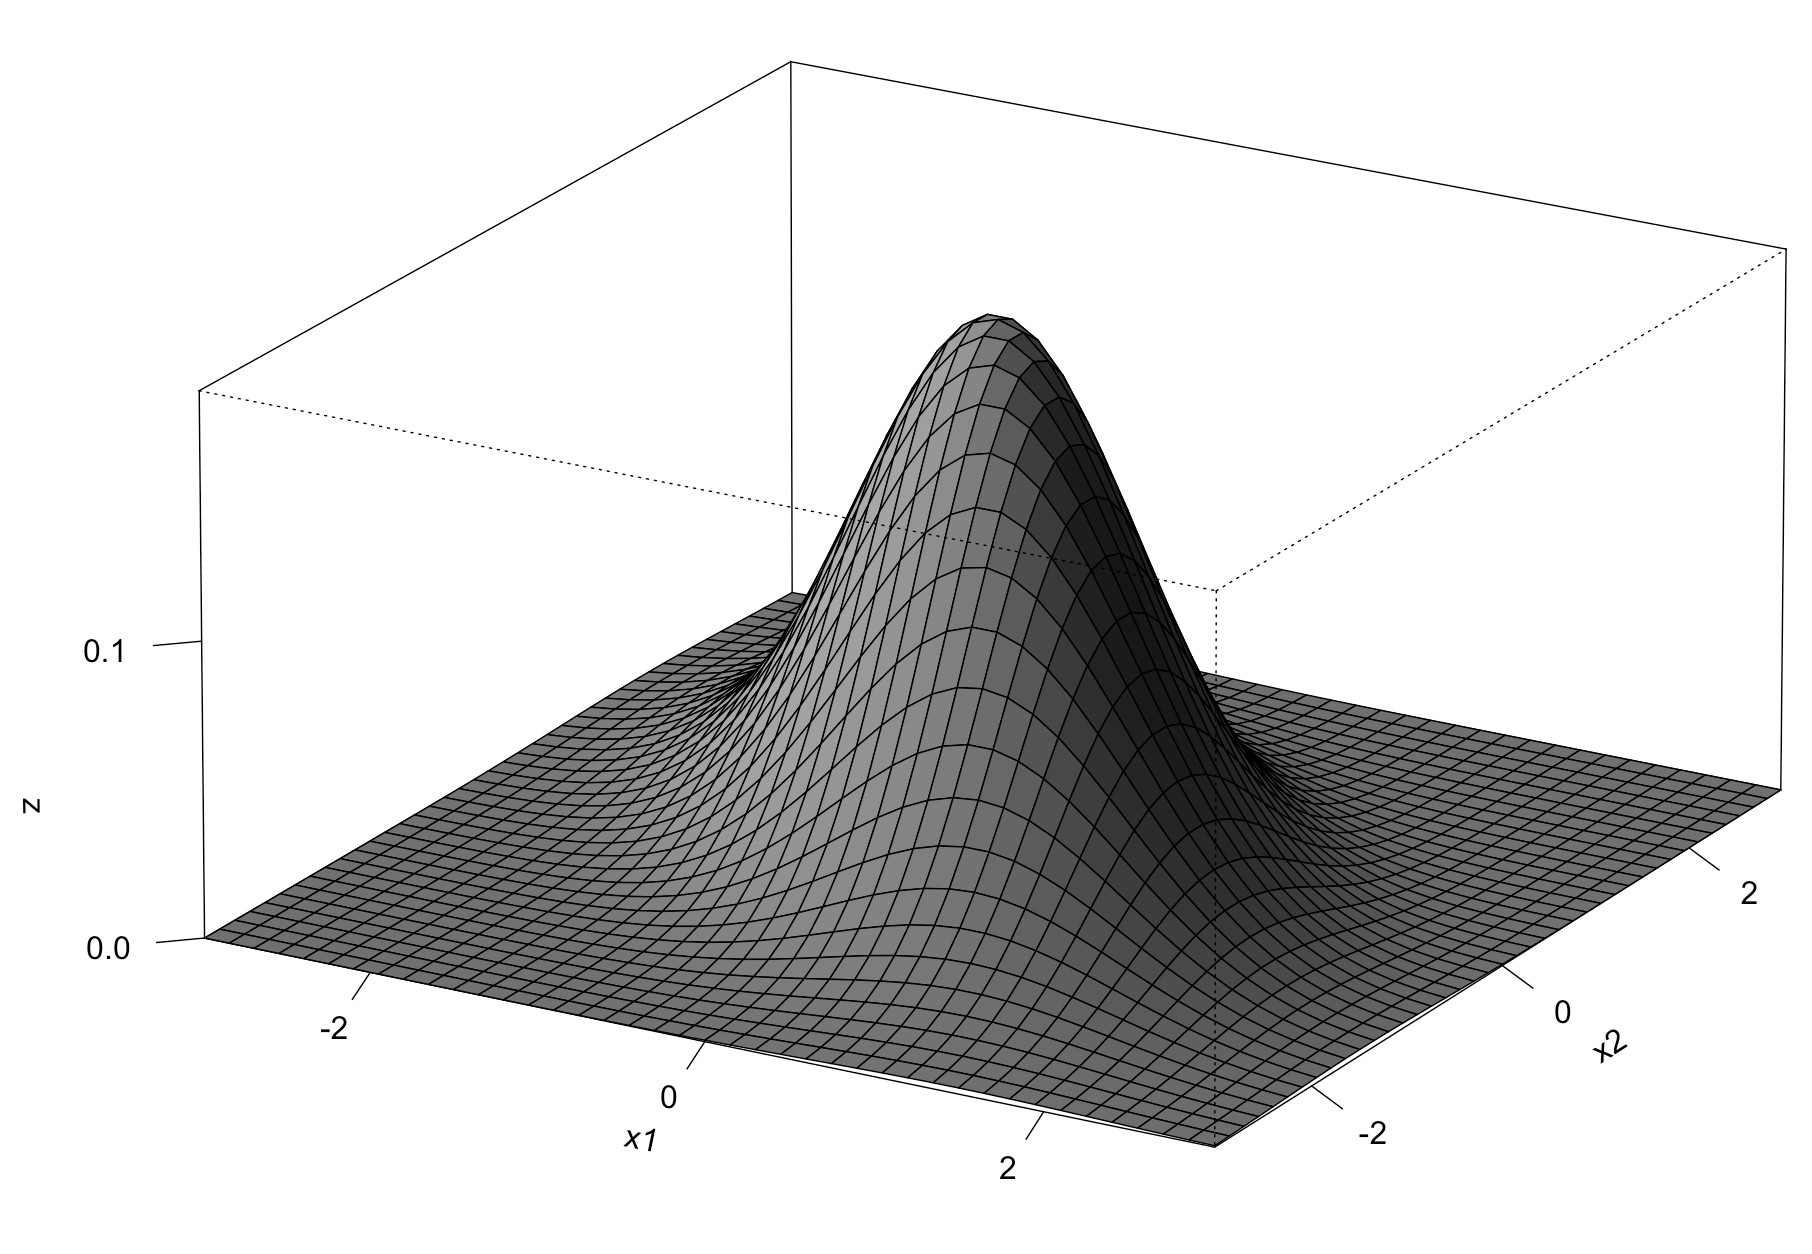
\includegraphics[width=0.5\linewidth,height=\textheight,keepaspectratio]{images/bivariate1.png}
\caption{Bivariate Normal Distribution}
\end{figure}

We won't work directly with the multivariate normal distribution, but there are some useful properties of normal random variables which we will use.

\begin{theorem}
If \(X \sim \mathcal{N}(\mu_X,\sigma^2_X)\) and \(Y \sim \mathcal{N}(\mu_Y,\sigma^2_Y)\), then:
\(X+Y \sim \mathcal{N}(\mu_X+\mu_Y,\sigma^2_X+\sigma^2_Y+2Cov(X,Y))\), that is, the sum of normal random variables is a normal random variable.
\end{theorem}

\begin{theorem}
If \(X \sim \mathcal{N}(\mu_X,\sigma^2_X)\) and \(Y \sim \mathcal{N}(\mu_Y,\sigma^2_Y)\) and X and Y are independent, then: \(X+Y \sim \mathcal{N}(\mu_X+\mu_Y,\sigma^2_X+\sigma^2_Y)\).
\end{theorem}

\begin{example}
Suppose \(X\) and \(Y\) are independent normal random variables with means \(\mu_X=2\) and \(\mu_Y=3\) and variances \(\sigma_X^2=1\) and \(\sigma_Y^2=4\). Determine the distribution of \(Z = 4X-Y\).
\end{example}

\vfill

\newpage

\section{R Companion for Chapter 5}\label{r-companion-for-chapter-5}

\begin{example}
Let's return to the Hubble dataset. Let's load the dataset into R and then plot the data. Note the plot parameter \textbf{pch=16} fills in the data points for a nicer looking plot.
\end{example}

\begin{Shaded}
\begin{Highlighting}[]
\NormalTok{hubble }\OtherTok{=} \FunctionTok{read\_csv}\NormalTok{(}\AttributeTok{file =} \StringTok{"hubble.csv"}\NormalTok{)}
\FunctionTok{plot}\NormalTok{(Velocity}\SpecialCharTok{\textasciitilde{}}\NormalTok{Distance,}\AttributeTok{data=}\NormalTok{hubble, }\AttributeTok{pch=}\DecValTok{16}\NormalTok{)}
\end{Highlighting}
\end{Shaded}

\begin{center}
\includegraphics[height=0.4\textheight]{_main_files/figure-latex/unnamed-chunk-92-1} \end{center}

There appears to be a positive relationship between Distance and Velocity. We can calculate the correlation and covariance between the two variables as well.

\begin{Shaded}
\begin{Highlighting}[]
\FunctionTok{cor}\NormalTok{(hubble}\SpecialCharTok{$}\NormalTok{Distance,hubble}\SpecialCharTok{$}\NormalTok{Velocity)}
\end{Highlighting}
\end{Shaded}

\begin{verbatim}
## [1] 0.789032
\end{verbatim}

\begin{Shaded}
\begin{Highlighting}[]
\FunctionTok{cov}\NormalTok{(hubble}\SpecialCharTok{$}\NormalTok{Distance,hubble}\SpecialCharTok{$}\NormalTok{Velocity)}
\end{Highlighting}
\end{Shaded}

\begin{verbatim}
## [1] 189.159
\end{verbatim}

The correlation is +0.789 indicating a positive, moderately strong linear relationship between Distance and Velocity. The covariance is 189.159 which is less interpretable since covariance is dependent on the units of measurement. For this reason, we typically prefer to use correlation rather than covariance.

\newpage

\begin{example}
The \textbf{mtcars} dataset is provided in the base version of R. To find out more info about this dataset, you can get details by calling \textbf{?mtcars}.
\end{example}

\begin{Shaded}
\begin{Highlighting}[]
\CommentTok{\# get info on the mtcars dataset}
\NormalTok{?mtcars}
\end{Highlighting}
\end{Shaded}

In the side window of R Studio, it should display the following description after running \textbf{?mtcars}.

The data were extracted from the 1974 Motor Trend US magazine, and comprises fuel consumption and 10 aspects of automobile design and performance for 32 automobiles (1973--74 models).

Let's load the dataset and take a look at the first few values.

\begin{Shaded}
\begin{Highlighting}[]
\FunctionTok{data}\NormalTok{(mtcars)}
\FunctionTok{head}\NormalTok{(mtcars)}
\end{Highlighting}
\end{Shaded}

\begin{verbatim}
##                    mpg cyl disp  hp drat    wt  qsec vs am gear carb
## Mazda RX4         21.0   6  160 110 3.90 2.620 16.46  0  1    4    4
## Mazda RX4 Wag     21.0   6  160 110 3.90 2.875 17.02  0  1    4    4
## Datsun 710        22.8   4  108  93 3.85 2.320 18.61  1  1    4    1
## Hornet 4 Drive    21.4   6  258 110 3.08 3.215 19.44  1  0    3    1
## Hornet Sportabout 18.7   8  360 175 3.15 3.440 17.02  0  0    3    2
## Valiant           18.1   6  225 105 2.76 3.460 20.22  1  0    3    1
\end{verbatim}

In the code below, we extract just these two variables from \textbf{mtcars} and create a new dataset \textbf{m}. From this new dataset \textbf{m}, we can construct a two-way table of counts for the combinations of \textbf{cyl} and \textbf{gear}.

\begin{Shaded}
\begin{Highlighting}[]
\CommentTok{\# creating new dataset m}
\NormalTok{m }\OtherTok{=}\NormalTok{ mtcars[ , }\FunctionTok{c}\NormalTok{(}\StringTok{"cyl"}\NormalTok{, }\StringTok{"gear"}\NormalTok{)]}

\CommentTok{\# construct a two{-}way table of counts for cyl and gear}
\NormalTok{m.table }\OtherTok{=} \FunctionTok{table}\NormalTok{(m}\SpecialCharTok{$}\NormalTok{cyl, m}\SpecialCharTok{$}\NormalTok{gear)}
\NormalTok{m.table}
\end{Highlighting}
\end{Shaded}

\begin{verbatim}
##    
##      3  4  5
##   4  1  8  2
##   6  2  4  1
##   8 12  0  2
\end{verbatim}

\newpage

We can also construct the joint probability mass function by dividing our table by the total number of observations.

\begin{Shaded}
\begin{Highlighting}[]
\CommentTok{\# calculate the number of total observations}
\NormalTok{n }\OtherTok{=} \FunctionTok{sum}\NormalTok{(m.table); n}
\end{Highlighting}
\end{Shaded}

\begin{verbatim}
## [1] 32
\end{verbatim}

\begin{Shaded}
\begin{Highlighting}[]
\CommentTok{\# construct the joint pmf}
\NormalTok{m.pmf }\OtherTok{=}\NormalTok{ m.table}\SpecialCharTok{/}\NormalTok{n; m.pmf}
\end{Highlighting}
\end{Shaded}

\begin{verbatim}
##    
##           3       4       5
##   4 0.03125 0.25000 0.06250
##   6 0.06250 0.12500 0.03125
##   8 0.37500 0.00000 0.06250
\end{verbatim}

Using the table, we can see that P(gear=3 and cyl=8) = 0.375 for example. What is P(gear=4 and cylinder = 4)? The middle entry of the table tells us this value is 0.125. In other words, 12.5\% of the cars in this dataset have 4 gears and 4 cylinders.

Next, we are going to look at the joint probability mass function (PMF) of the variables \textbf{cyl} and \textbf{gear}. We can get the marginal PMFs by summing across rows and columns of the joint pmf.

\begin{Shaded}
\begin{Highlighting}[]
\CommentTok{\# marginal pmf of gear}
\FunctionTok{colSums}\NormalTok{(m.pmf)}
\end{Highlighting}
\end{Shaded}

\begin{verbatim}
##       3       4       5 
## 0.46875 0.37500 0.15625
\end{verbatim}

\begin{Shaded}
\begin{Highlighting}[]
\CommentTok{\# marginal pmf of cyl}
\FunctionTok{rowSums}\NormalTok{(m.pmf)}
\end{Highlighting}
\end{Shaded}

\begin{verbatim}
##       4       6       8 
## 0.34375 0.21875 0.43750
\end{verbatim}

From the tables above, you should see that P(gear=3)=0.46875 and P(cyl=4)=0.34375.

Finally, we can get the correlation as follows. Note that gear and cyl have a negative, moderate linear relationship.

\begin{Shaded}
\begin{Highlighting}[]
\FunctionTok{cor}\NormalTok{(m}\SpecialCharTok{$}\NormalTok{cyl,m}\SpecialCharTok{$}\NormalTok{gear)}
\end{Highlighting}
\end{Shaded}

\begin{verbatim}
## [1] -0.4926866
\end{verbatim}

  \bibliography{book.bib,packages.bib}

\end{document}
